\begin{fullwidth}
\chapter{Structured priors for analyzing brain data: the models and algorithms}\label{chap:hrf_estimation}
\end{fullwidth}
\markright{{~{\rm \ref{chap:hrf_estimation}}. Data-driven HRF estimation}\hfill}{}

\section{SpaceNet: spatial priors for brain analysis}
Sparsity- and structure-inducing priors are used to
perform jointly the prediction of a target variable and region
segmentation in multivariate analysis settings.
%
Specifically, it has been shown that one can employ priors like Total
Variation (TV)  \cite{michel2011tv}, TV-$\ell_1$
 \cite{baldassarre2012,gramfort2013}, TV-ElasticNet
 \cite{dubois2014predictive},
and GraphNet  \cite{grosenick2013}
(aka Smooth-Lasso  \cite{hebiri2011})
%\footnote{Henceforth, we will use GraphNet and S-Lasso
%interchangeably.}
to regularize regression and classification
problems in brain imaging.
%

\begin{marginfigure}[4cm]
  \centering
  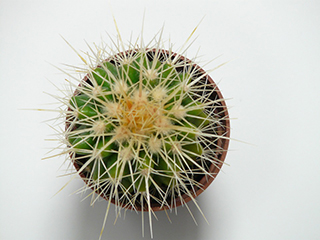
\includegraphics[width=1\linewidth]{figures/ball.jpg}
  \caption{$\ell_p$ ball with $0 < p \ll 1$.}
  \label{fig:roi}
\end{marginfigure}

We denote by ${\y} \in \mathbb{R}^{n}$ the targets to
be predicted (age, sex, IQ, etc.); the \textit{design matrix}
${\X}\in\mathbb{R}^{n \times p}$ are the
brain images related to the presentation of different
stimuli, or other brain acquisition (e.g gray-matter concentration
maps from anatomy, etc.). The integer $p$ is the number of voxels,
and $n$ the number of samples (images). In brain imaging, $n \ll p$;
typically, $p \sim 10^3-10^6$ (in full-brain analysis),
while $n \sim 10-10^3$ ($n$ being limited by the cost of acquisition,
etc.). $\nabla_x$ will denote the discrete spatial gradient operator
along the $x$-axis, $\nabla_y$ along the $y$-axis, etc.

\begin{marginfigure}[4cm]
  \centering
  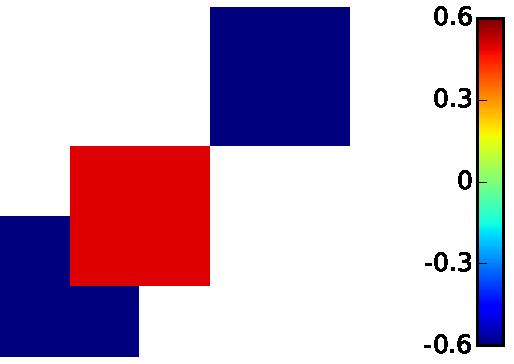
\includegraphics[width=.7\linewidth]{figures/cartoon.pdf}
  \caption{A cartoon showing a sparse and blobby brain map,
  as would be sought for by SpaceNet models \eqref{eq:ss}.}
  \label{fig:roi}
\end{marginfigure}
%\begin{marginfigure}[4cm]


%% Let $\Omega \subset \mathbb{R}^3$ be
%% the 3D image domain representing the region occupied by the brain --or
%% ROI (region of interest) thereof-- under  study, discretized regularly
%% on a finite grid.

Over time, a number of spatially regularized linear models have been proposed. These are mainly: Total-Variation (TV)
   \citep{michel2011tv}, TV-$\ell_1$  \citep{baldassarre2012,gramfort2013}, GraphNet  \citep{grosenick2013,hebiri2011},
  TV-ElasticNet  \citep{dubois2014predictive}, Sparse Variation  \citep{eickenberg2015total}, and social-sparsity  \citep{kowalski2013social}. These can all be written in a general framework as follows

\begin{equation}
  \underset{\w \in \mathbb R^p}{\text{minimize }}E(\w) := \ell(\y,\X\w) + \alpha \Omega(\nabla_\tau\w).
    \label{eq:opt_pb}
\end{equation}
The coefficients ${\w}$ define a spatial map in over the brain (one value per voxel).
$\Omega \circ \nabla_\tau$ is the penalty term ($\nabla_\tau$ is the extended discrete gradient operator defined in equation \eqref{eq:extau} of section{sec:notation}), which simultaneously imposes both sparsity and structure (blobs). The different spatial regularization
methods that have appeared in neuro-imaging literature can be cast into this
correspond to different choices of the convex penalty $\Omega$ acting on the extended gradient of the coefficients $\w$. Viz,
\[
  \begin{split}
  \Omega(\z) = \begin{cases}
      \|\z_4\|_1 + \frac{1}{2}\|\z_{1:3}\|_{\text{Fro}}^2 := \sum_{j=1}^p|\z_{4,j}| + \frac{1}{2}\sum_{j=1}^{p}\sum_{k=1}^3\z_{k,j}^2, &\mbox{ GraphNet \citep{grosenick2013,hebiri2011}},\\\\
      \|\z_4\|_1 + \|\z_{1:3}\|_{2,1} := \sum_{j=1}^p|\z_{4,j}| + \sum_{j=1}^{p}\sqrt{\sum_{k=1}^3\z_{k,j}^2}, &\mbox{ for TV-$\ell_1$ \citep{baldassarre2012,gramfort2013}},\\
      \|\z\|_{2,1} = \sum_{j=1}^{p}\sqrt{\sum_{k=1}^4\z_{k,j}^2}, &\mbox{ for Sparse Variation \citep{eickenberg2015total}},\\
      ...
    \end{cases}
  \end{split}
\]
{$\alpha > 0$} controls the total amount of regularization, while
  {$\tau$
    ($0 < \tau \le 1$)} is a
  mixing constant between
  the {sparsity-inducing} $\ell_1$ part and the
  {cluster-promoting} part of the penalty term.
  The particular case {$\tau = 1$} corresponds to the usual Lasso. Vanilla TV  \citep{michel2011tv} corresponds to TV-$\ell_1$ with $\tau = 0$.
The term {$\ell(\y,\X\w)$} is the
  {loss / data-fit term}. Popular choices include:
  $$
  \ell(\y,\X\w) = \frac{1}{n}\begin{cases}\frac{1}{2}\|\X\w - \y\|_2^2 = \frac{1}{2}\sum_{i=1}^n(\X^T_i\w - \y_i)^2,
    &\mbox{ \text{ for least-squares (e.g in regression settings)}}\\
    \sum_{i=1}^n \log(1+\exp(-\y_i\X_i^T\w)),
    &\mbox{ \text{ for logistic regression (e.g in classification)}},\\\ldots\end{cases}$$

 \begin{figure}[!htb] 
  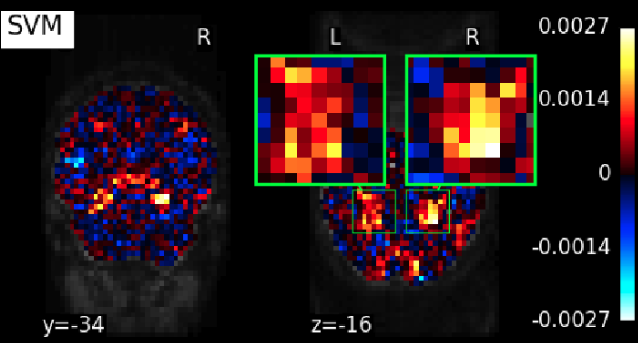
\includegraphics[width=.325\linewidth]{figures/svm.png}
  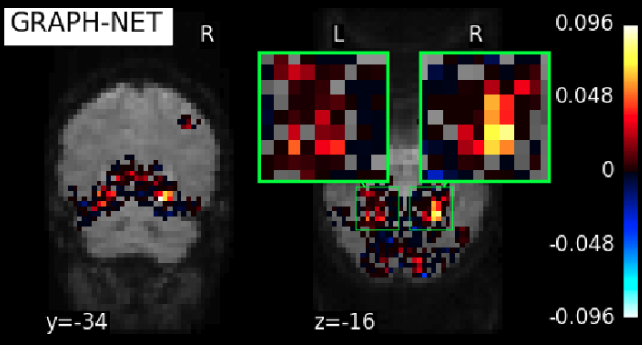
\includegraphics[width=.325\linewidth]{figures/graphnet.png}
  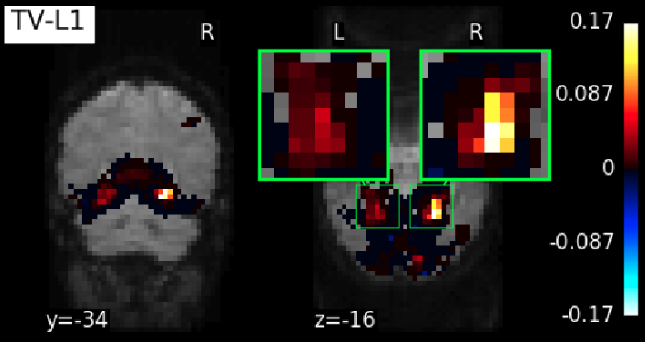
\includegraphics[width=.325\linewidth]{figures/tvl1.png}  
  \caption{The figure shows results of comparing the SpaceNet  models TV-$\ell_1$ and
    Graph-Net against an SVM (Support Vector Machine) classifier on
    the visual-recognition dataset  \citep{haxby2001}
    As can be seen from the figure, SpaceNet priors (TV-$\ell_1$, GraphNet, etc.)
    yield stable and more intepretable maps. Figure taken from OHBM
    presentation  \citep{spacenetohbm}.}
  \label{fig:spacenet_maps}
%  \end{marginfigure}
\end{figure}
  The result of such regularized models, dubbed \emph{SpaceNet}
 \citep{spacenetohbm}, are brain maps which are both
sparse (i.e regression coefficients $\w$ are zero everywhere, except at
predictive voxels) and structured (blobby). The superiority of such
methods over methods without structured priors like the Lasso, ANOVA,
Ridge, SVM, etc. for yielding more intepretable maps and improved
prediction scores is now well established. See for example
 \citep{baldassarre2012,gramfort2013}. These priors are fast becoming
popular for brain decoding and segmentation. Indeed, they leverage a
feature-selection function
(since they limit the number of active voxels),
and also a structuring function
(since they penalize local
differences in the values of the brain map). For example, see Fig.
\ref{fig:spacenet_maps}.
Also, such priors produce state-of-the-art methods for automatic
extraction of functional brain atlases  \citep{abraham2013}.
  
%%  \citep{dohmatob2015spacenet}, \citep{abraham2013}, \citep{abrahamregion},
%%  \citep{eickenberg2015total},
\section{Efficient optimization of sparsity and smoothness regularized models}
Though the SpaceNet model presented above leads to superior estimators compared to classical estimators (Ridge regression, SVM, etc.) without spatial penalization, it is considerably harder to optimize than these classical models. Indeed, the corresponding optimization problems is non-separable in the model coefficients, and except for the case of GraphNet,
the penalty term $\Omega \circ \nabla_\tau$ is neither smooth nor proximable.
\footnote{ A function $f$ is said to be \textit{proximable} is the operator $\text{prox}_{\gamma f}$ is easy to compute. This is the case for $\ell_p$-norms  (with $ p \ge 1$, to ensure convexity) and indicator functions of simple closed convex sets like balls, simplexes, half-spaces, etc.}
For the penalty to fully exercise its
\begin{figure}[!htb]
    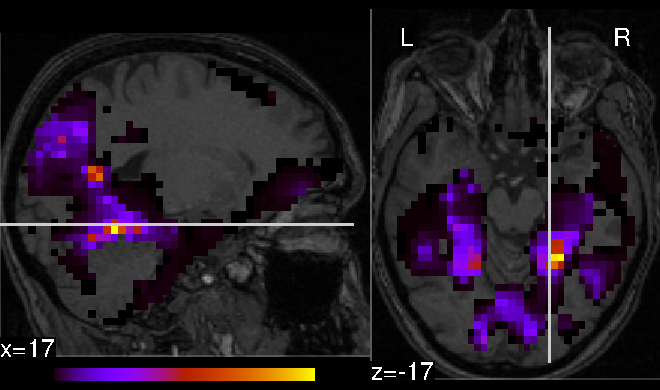
\includegraphics[width=.331\linewidth]{face_vs_house_tol_0_1.pdf}%
\llap{\color{white}\raisebox{.17\linewidth}{\rlap{\sffamily Stopping:
      $\Delta E < 10^{-1}$}}\hspace*{.315\linewidth}}\hfill%
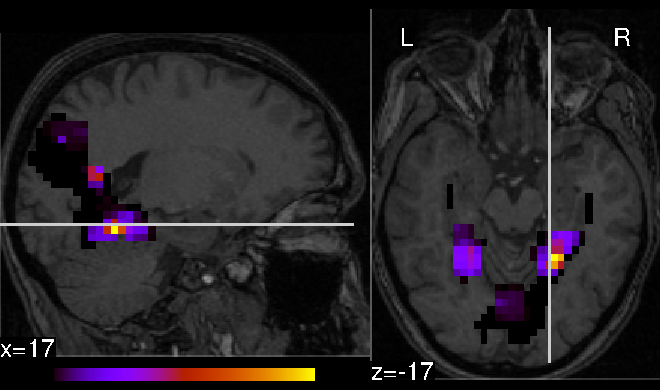
\includegraphics[width=.331\linewidth]{face_vs_house_tol_0_001.pdf}%
\llap{\color{white}\raisebox{.17\linewidth}{\rlap{\sffamily Stopping:
      $\Delta E < 10^{-3}$}}\hspace*{.315\linewidth}}\hfill%
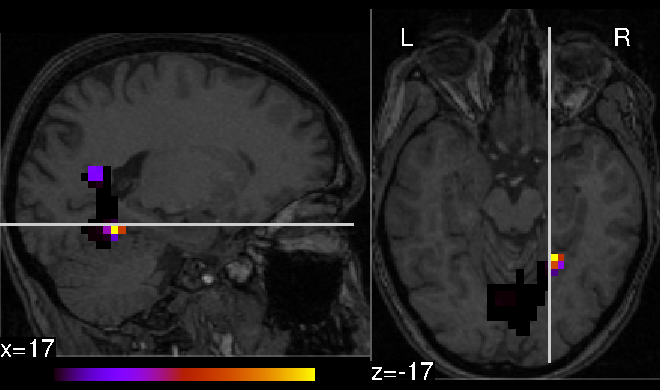
\includegraphics[width=.331\linewidth]{face_vs_house_tol_1e-05.pdf}%
\llap{\color{white}\raisebox{.17\linewidth}{\rlap{\sffamily Stopping:
      $\Delta E < 10^{-5}$}}\hspace*{.315\linewidth}}%

\caption{TV-$\ell_1$ maps for the face-house discrimination task on
  the visual recognition dataset.
  Note that
  the stopping criterion is defined as a threshold on the energy
  decrease per one iteration of the algorithm, and thus differs from
  the tolerance displayed in figure \ref{Fig:benchmarks_prni}.  This figure shows
  the importance of convergence for problem \eqref{eq:opt_pb}, and motivates
  the need for fast solvers for SpaceNet priors, especially the non-smooth ones like TV-$\ell_1$ and Sparse Variation. See the full story in
 \citep{dohmatob2014benchmarking}}
  \label{Fig:benchmarks_prni}
\end{figure}

structuring effect on the maps, this optimization problem must be
solved to a good tolerance resulting in a computational challenge. Lack of good solver and explicit control of
tolerance can lead to brain maps and conclusions that reflect
properties of the solver more than of model coefficients, as illustrated in Fig. \ref{Fig:benchmarks_prni}.
In our prize-winning PRNI paper  \citep{dohmatob2014benchmarking}, we did an extensive study of all solvers applicable to the problem in TV-$\ell_1$ special case (which happens to be the most difficult scenario).
Our results outlined the best strategy: a double FISTA loop, where the
inner loop computes the proximal operator of the penalty term, with approximate precision on the duality-gap. This was
further refined and implemented in  \citep{varoquaux2015faasta}.

  %% \begin{itemize}
  %% \item{proximal methods}
  %%   \begin{itemize}
  %%     \item single-step\\
  %%       {-} ISTA (Iterative Soft-Thresholding Algorithm)  \citep{daubechies2004}
  %%     \item multi-step / accelerated\\
  %%       {-} FISTA (Fast ISTA)  \citep{beck09fista}
  %%   \end{itemize}
  %% \item {primal-dual \& splitting methods}
  %%   \begin{itemize}
  %%   \item ADMM (Alternating Directions Method of Multipliers)  \citep{boyd2011distributed}
  %%     % (\textit{Alternating Directions Method of Multipliers})
  %%   \item Chambolle-Pock's Primal-Dual  \citep{chambolle2010}
  %%   \end{itemize}
  %% \item {quasi-Newton methods}
  %%   \begin{itemize}
  %%   \item HANSO ({Hybrid Algorithm for Non-smooth Optimization})  \citep{lewis2008}
  %%   \item L-BFGS  \citep{ciyou1994} on smooth surrogates of the penalty
  %%   \end{itemize}
  %% \end{itemize}
  

%% \begin{figure*}
%%   \begin{subfigure}[t]{1\linewidth}
%%     \hspace*{-.01\linewidth}%
%%     \includegraphics[width=.6\linewidth]{haxby_lr_energy.pdf}
%%     \hspace*{-.09\linewidth}%
%%     \includegraphics[width=.6\linewidth]{haxby_lr.pdf}%
%%     % \vspace{-2ex}
%%     \caption{\textbf{Classification} with logistic regression model
%%       \eqref{eq:opt_pb}. on the visual recognition face-house
%%     discrimination task. \textbf{Left}: excess energy $E(\mathbf{w}_t) -
%%     E(\mathbf{w})_{t \rightarrow \infty}$ as a function 
%%     of time.
%%     \textbf{Right}: convergence time of the various solvers for different
%%     choice of regularization parameters.
%%     Broken lines correspond to a tolerance of $10^{0}$,
%%     whilst full-lines correspond to $10^{-2}$.  The thick vertical line
%%     indicates the best model selected by cross-validation.}
%%     \label{Fig:HaxbyLR}
%%   \end{subfigure}
%%   \begin{subfigure}[t]{1\linewidth}
%%     \includegraphics[width=.6\linewidth]{haxby_mse.pdf}%
%%     \hspace{-.09\linewidth}%
%%     % generate with: ipython ../wip/tv_l1_solver/plot_parallel_plots.py poldrack_mse_12th.json 2e1 --pdb
%%     \includegraphics[width=.6\linewidth]{poldrack_mse.pdf}
%%     % \vspace{-2ex}
%%     \caption{\textbf{Regression.} results. \textbf{Left}:
%%       on the visual recognition  face-house discrimination task; \textbf{Right}: on the
%%       Mixed gambles dataset. Broken lines correspond to a tolerance of $10^{0}$,
%%       whilst full-lines correspond to $10^{-2}$. The thick vertical line
%%       indicates the best model selected by cross-validation.}
%%     \label{Fig:MSEtimes}
%%   \end{subfigure}
%% \caption{Benchmarks for different solvers for the TV-$\ell_1$ model
%%   \eqref{eq:opt_pb} on the visual recognition face-house
%%   discrimination task. See  \citep{dohmatob2014benchmarking} for more details.}
%% \end{figure*}

\section{Choice of solver}
Learning predictive models from brain imaging
data, as in decoding cognitive states from fMRI (functional Mag-
netic Resonance Imaging), is typically an ill-posed problem as it
entails estimating many more parameters than available sample
points.
 \begin{figure}[!htbp]
   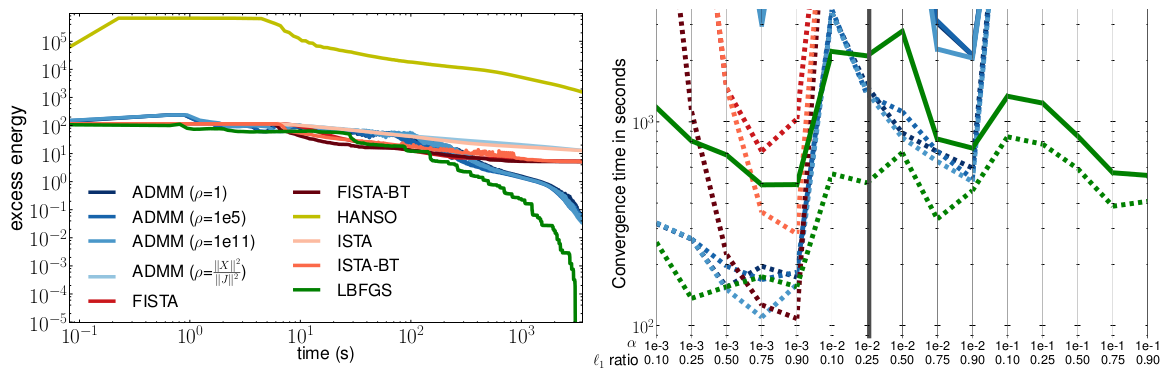
\includegraphics[width=1\linewidth]{figures/solvers_1.png}
   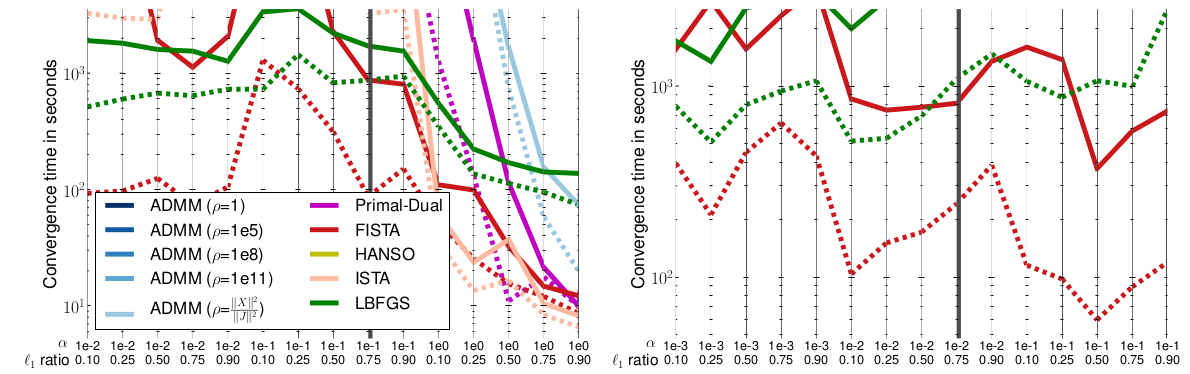
\includegraphics[width=1\linewidth]{figures/solvers_2.png}
   \caption{\textbf{Benchmarking } solvers for TV-$\ell_1$ penalized models. \textbf{Top:} TV-$\ell_1$ penalized Logistic Regression on the visual recognition face-house discrimination task. \textbf{Top Left:} excess energy $E(\B{w}_t ) - E(\B{w}^*)$ as a function of time. \textbf{Top Right:} convergence time of the various solvers for different choice of regularization parameters. Broken lines correspond to a tolerance of
$10^0$ , whilst full-lines correspond to $10^{-2}$ . The thick vertical line indicates the best model selected by cross-validation. \textbf{Bottom:} TV-$\ell_1$ penalized Least-Squares Regression. \textbf{Bottom Left:} on the visual recognition face-house discrimination task; \textbf{Bottom Right:} on the Mixed gambles dataset. The thick vertical line indicates the best model selected by cross-validation.}
\end{figure}
This estimation problem thus requires regularization.
Total variation regularization, combined with sparse models, has
been shown to yield good predictive performance, as well as stable
and interpretable maps. However, the corresponding optimization
problem is very challenging: it is non-smooth, non-separable
and heavily ill-conditioned. For the penalty to fully exercise its
structuring effect on the maps, this optimization problem must be
solved to a good tolerance resulting in a computational challenge.
Here we explore a wide variety of solvers and exhibit their
convergence properties on fMRI data.
We introduce a variant
of smooth solvers and show that it is a promising approach in
these settings. Our findings show that care must be taken in
solving TV-$\ell_1$ estimation in brain imaging and highlight the
successful strategies.

\paragraph{Results of empirical benchmarks.}
Our results outline best strategies: monotonous FISTA with
a adaptive control of the tolerance of the TV proximal op-
erator, in the case of squared loss; smoothed quasi-newton
based on surrogate upper-bounds of the non-smooth norms for
logistic loss. While these algorithms are variants of existing
approaches, we present here novel additions useful for the
TV or TV-$\ell_1$ settings. The fact that the smooth approaches
emerge as fast solvers on these non-smooth problems is not
unexpected as i) the amount of regularization is small ii) the
prevailing term is smooth and very ill conditioned, thus calling
for second-order methods such as Newton or quasi-Newton.
For neuroimaging applications, our study has highlighted
the need to converge to a good tolerance and the correspond-
ing difficulties. Lack of good solver and explicit control of
tolerance can lead to brain maps and conclusions that reflect
properties of the solver more than of the TV-$\ell_1$ solution.

\section{More speed via univariate feature-screening and early-stopping}
In our PRNI 2015 conference paper  \citep{dohmatob2015speeding}, we presented some heuristics for speeding up the overall optimization process: (a) Early-stopping, whereby one  halts
the optimization process when the test score (performance on left-out
data) for the internal cross-validation for model-selection stops
improving, and (b) univariate feature-screening, whereby irrelevant
(non-predictive) voxels are detected and eliminated before the
optimization problem is entered, thus reducing the size of the
problem.

Empirical results with GraphNet on real MRI (Magnetic
Resonance Imaging)
datasets indicate that these heuristics are a win-win strategy, as
they add speed without sacrificing the quality of the predictions
/ classifications.

 \begin{figure}[!htb]
   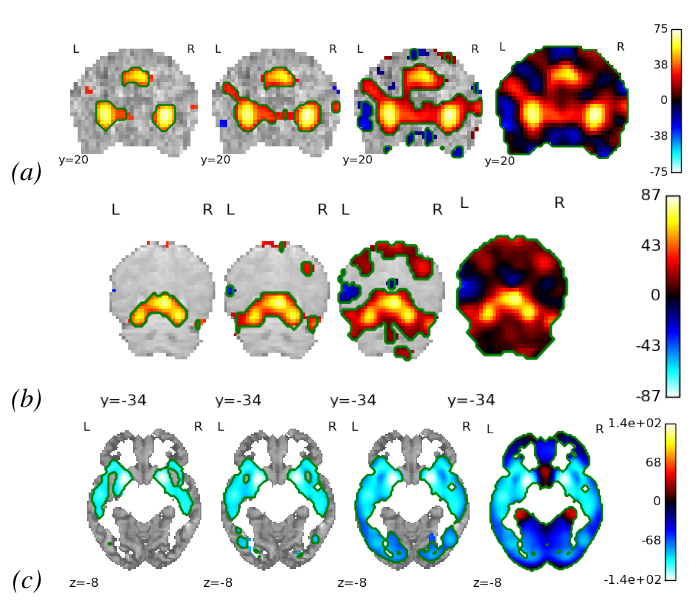
\includegraphics[width=1\linewidth]{figures/screening.png}
\caption{Univariate feature-screening for the
  GraphNet
  % \citep{hebiri2011,grosenick2013}
  problem \eqref{eq:opt_pb} on
  different datasets.
  % $(X,y)$.
  This figure shows spatial maps of
  $X^T_jy$, thresholded so that only voxels $j$ with (from left to
  rightmost column)  $|X^T_jy| \ge p_{10\%}(|X^Ty|)$, $|X^T_jy| \ge
  p_{20\%}(|X^Ty|)$, $|X^T_jy| \ge p_{50\%}(|X^Ty|)$, and $|X^T_jy|
  \ge p_{100\%}(|X^Ty|)$ (full-brain) respectively, survive. The
  green contours enclose the elite voxels which are selected by the
  screening procedure at the respective threshold
  levels. \textit{(a)}: Mixed Gambles dataset
  \citep{jimura2012}.%  Remarkably, the geometry of the regions obtained
  % here for the 10th and 20th screening-percentiles match pretty well
  % the results obtained in \citep{gramfort2013} with their TV-L1
  % penalty. \textit{(b)}: Face vs House contrast of the visual recognition
  % dataset \citep{haxby2001}. 
  Weights maps obtained for the GraphNet
  model \eqref{eq:opt_pb} with these different
  screening-percentiles are shown in Figure
  \ref{fig:haxby}. \textit{(c)}: OASIS dataset \citep{marcus2007open}
  with VBM. See Figure \ref{fig:oasis} for weights maps and
  age predictions obtained using these different
  screening-percentiles. % on the GraphNet model \eqref{eq:opt_pb}.
}

\label{fig:screening}
\end{figure}

\subsection{Methods}
%% We will now detail the heuristic techiques for speeding up
%% numerical optimization of GraphNet \citep{hebiri2011,grosenick2013}
%% model for brain data.


\paragraph{A note on implementation of the solver.}
One notes that in the penalty term $J(w)$ of problem
\eqref{eq:opt_pb}, the $\|\nabla
w\|^2_2$ sub-term is smooth (i.e differentiable) with
\textit{Lipschitz} gradient, whilst the $\ell_{1}$ term though
nonsmooth, is \textit{proximable}\footnote{That is, there is a
  closed-form analytic expression for its proximal operator.} by means
of the \textit{soft-thesholding} operator \citep{daubechies2004}.  Thus
problem \eqref{eq:opt_pb} is amenable to the FISTA (Fast Iterative
Shrinkage-Thresholding Algorithm) \citep{beck09fista}, with a provable
$\mathcal{O}(1/\sqrt{\epsilon})$ convergence rate. Our implementation
of FISTA uses technical recommendations
(line-searching, parametrization, etc.) which were provided in
\citep{dohmatob2014benchmarking}, in the context of TV-L1
\citep{baldassarre2012,gramfort2013}. The model parameters $\alpha$ and
$\rho$ in \eqref{eq:opt_pb} are set by \textit{internal}
cross-validation.

%% \paragraph*{(b) Warm-start}
%% The $(\alpha, \rho)$ parameter grid is walked $\rho$-first. For each $\rho$ value encountered, the alphas are walked from largest to smallest value. The largest value is contructed to be the largest value of $\alpha$ for which the optimal solution to problem \eqref{eq:opt_pb} is necessarily zero.

%% We now provide details on the speedup heuristics for speeding up
%% the overall implementation, including model-selection part of it.


\paragraph{Univariate feature-screening.}
%% \textbf{XXX: In a paragraph briefly give a comprehensive overview of
%%   screening algorithms and heuristics from El Ghaoui, upto the more
%%   recent Liu et al!!!}
In machine-learning, feature-screening aims at detecting and
eliminating irrelevant (non-predictive)
features thus reducing the size of the underlying
optimization problem (here problem \eqref{eq:opt_pb}). The general idea
is to compute for each value of the regularization parameter, a
\textit{relevance measure} for each feature, which is then compared with a
threshold (produced by the screening procedure itself). Features which fall short
of this threshold are detected as irrelevant and eliminated. For the
Lasso and similar models (including Group Lasso),
\textit{exact}\footnote{i.e, techniques
  which don't mistakenly discard active predictive features.}
screening techniques include those developed in
\citep{elghaoui2010,lee2014exact,liu2014safe,wang2015lasso}. Inexact
screening techniques (e.g \citep{tibshirani2010strong}) have also been
proposed in the literature.
Our proposed heuristic screening technique is inspired by the
\textit{Marginal screening} technique developed in Algorithm 1 of
\citep{lee2014exact}, and operates as
follows. The data $(X,y)$ are standardized so that $y$ has unit
variance and zero mean, likewise each row of the design matrix $X$. To
ensure obtention of a smooth mask, a Gaussian-smoothed version
of $X$ is used in the screening procedure (but not in the actual model
fit).
For each voxel $j$ (voxels are the features here) the
absolute dot-product $|X^T_jy|$ of $y$ with the $j$th column of
$X$ is computed.
% This is used as the relevance measure.
For a given screening-percentile
$sp \in [0, 100]$ , the $sp$th percentile value of the
vector $|X^Ty| := (|X^T_1y|, ..., |X^T_py|)$, denoted $p_{sp}(|X^Ty|)$,
is computed. The case $sp=100$ corresponds to full-brain analysis. 25
means we keep the quarter of the brain made of voxels with the highest
$|X^T_jy|$ values, and so on.
% ; this is the threshold.
A brain-mask is then formed containing only those voxels $j$
for which $|X^T_jy| \ge p_{sp}(|X^Ty|)$. Next, this brain-mask is
morphologically eroded
% (to remove isolated small patches)
and then
dilated, to obtain a more structured mask.  Figure
\ref{fig:screening} shows results of applying this screening heuristic
to various datasets, prior to model fitting.

\subsection{Experiments}
We experimented our early-stopping and (separately)
feature-screening heuristics on different MRI datasets.
All experiments were run using a single core of
  a laptop.

\paragraph{Regression.} The OASIS dataset
    \citep{marcus2007open} consists of a
    cross-sectional collection of 416 subjects aged 18 to 96. For each
    subject, 3 or 4 individual T1-weighted MRI scans obtained in
    single scan sessions are included.   A natural regression problem
    for this dataset is to predict the age of a subject from their
    anatomical data. To this end, we segmented the gray-matter from
    the anatomy of each subject (obtained from the T1 images), and
    used the gray-matter maps
    as features for predicting age. We split the 416 subjects into two
    equally-sized and age-balanced groups: a train set and a validation
    set. The GraphNet model \citep{hebiri2011,grosenick2013} was fitted
    on the train set, with parameters
    ($\alpha$ and $\rho$ in \eqref{eq:opt_pb}) set internally via 8-fold
    cross-validation. The results for this experiment are shown in
    Figure \ref{fig:oasis}.

\paragraph{Classification.} The visual
    recognition dataset \citep{haxby2001} is a popular block-design
    fMRI dataset from a
    study on face and object representation in human ventral temporal
    cortex.
It consists of 6 subjects with 12 runs per subject. In each run, the
subjects
passively viewed images of eight object categories, grouped
in 24-second blocks separated by intermittent rest periods. This
experiment is a classification task: predicting the object category
$y$. We use a \textit{One-versus-Rest (OvR)} strategy. The design
matrix ${X}$ is made of
time-series from the full-brain mask of $p = 23\,707$ voxels over $n =
216$ TRs, of a single subject (subj1). We divided the 12 runs into 6
runs for training and 6 other runs for
validation. \textit{Leave-one-label-out} cross-validation was used for
selecting the model parameters $(\alpha, \rho)$. The results are
depicted in Figure \ref{fig:haxby}.

 \begin{figure}[!htb]
   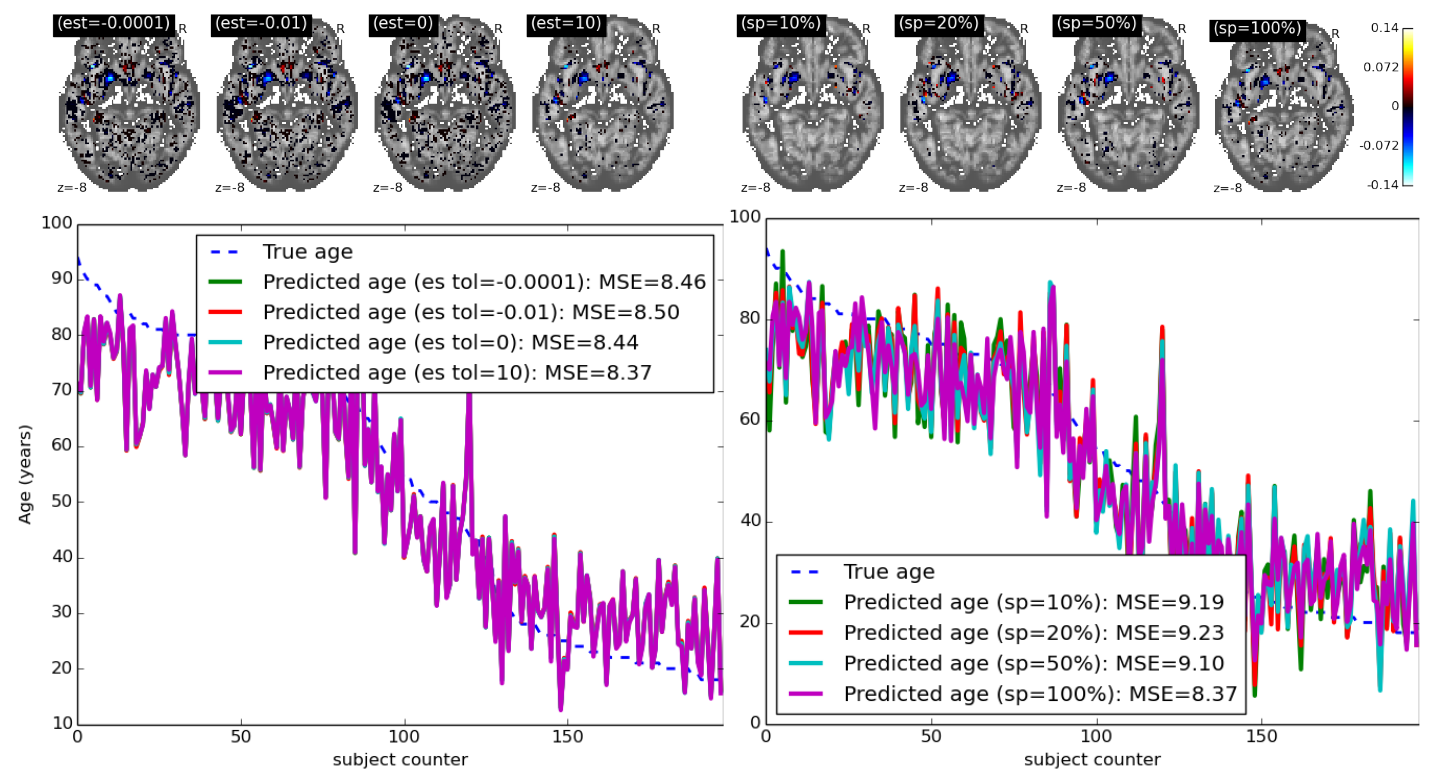
\includegraphics[width=1\linewidth]{figures/screening_weights.png}
  \caption{Predicting age from gray-matter concentration maps from the
    OASIS dataset \citep{marcus2007open}. \textbf{Top}:
    Weights maps (solutions to problem \eqref{eq:opt_pb}).
% \textbf{N.B}: The long spiky undershoots in the prediction curves
% are indicative of outliers: subjects for which spatial preprocessing
% (tissue segmentation, normalization, etc.) failed.
\textbf{Bottom-left}: Mean Square Error (MSE) in age prediction, for
different subjects of the validation set, for  varying levels of the
early-stopping tolerance (``es tol'' for short), with the
screening-percentile (sp) held constant at 100
(full-brain). \textbf{Bottom-right}: MSE in age prediction, for
varying levels of the screening-percentile (sp).%  \textbf{Running
%   times}: Increasing \textit{est tol} (from $-10^{-4}$ to $10$): \textbf{100.2m, 171.4m, 188.8m, 289.6m}. For
% increasing $sp$ ($10$ to $100$): \textbf{44.2m, 81.3m, 186.5m, 341.3m}
}   
\label{fig:oasis}
\end{figure}

\subsection{Results.}
We now summarize and comment the results of the experiments (refer to
section \ref{sec:experiments}).
Figure \ref{fig:oasis} shows the effects of early-stopping heuristic
and feature-screening heuristic on age prediction scores on the OASIS
dataset \citep{marcus2007open} (416 subjects). We see that in the
internal cross-validation, stopping  the optimization procedure for
fixed $(\alpha, \rho)$ pair of regularization parameters, when test
score increases by $-10^{-2}$ or more is a good heuristic, and does just
as good as running the optimization until numerical convergence. 
Also (and independently), one gets similar prediction scores using as
little as a fifth of the brain volume ($sp=20$),
compared to using the full-brain ($sp=100$).
Figure \ref{fig:haxby} reports similar results for classification on
the visual recognition dataset \citep{haxby2001}. Overall, we see from
Figures \ref{fig:haxby} and \ref{fig:oasis} that we can achieve upto
$10$-fold speedup with the proposed heuristics, with very little loss
in accuracy. Also, we see that contiguous groups of bars are roughly flat at the top, with a
    sligh increase from lower to high screening-percentile values. The
    case ``chair vs scramped'' is an exception, where a slightly reverse tendency
    if observed. A possible explanation is that $20$th percentile
    feature-screening already selects the right voxels (quasi-exact
    support recovery), and so including more voxels in the model can only hurt its
    performance...    

 \begin{figure}[!htb]
   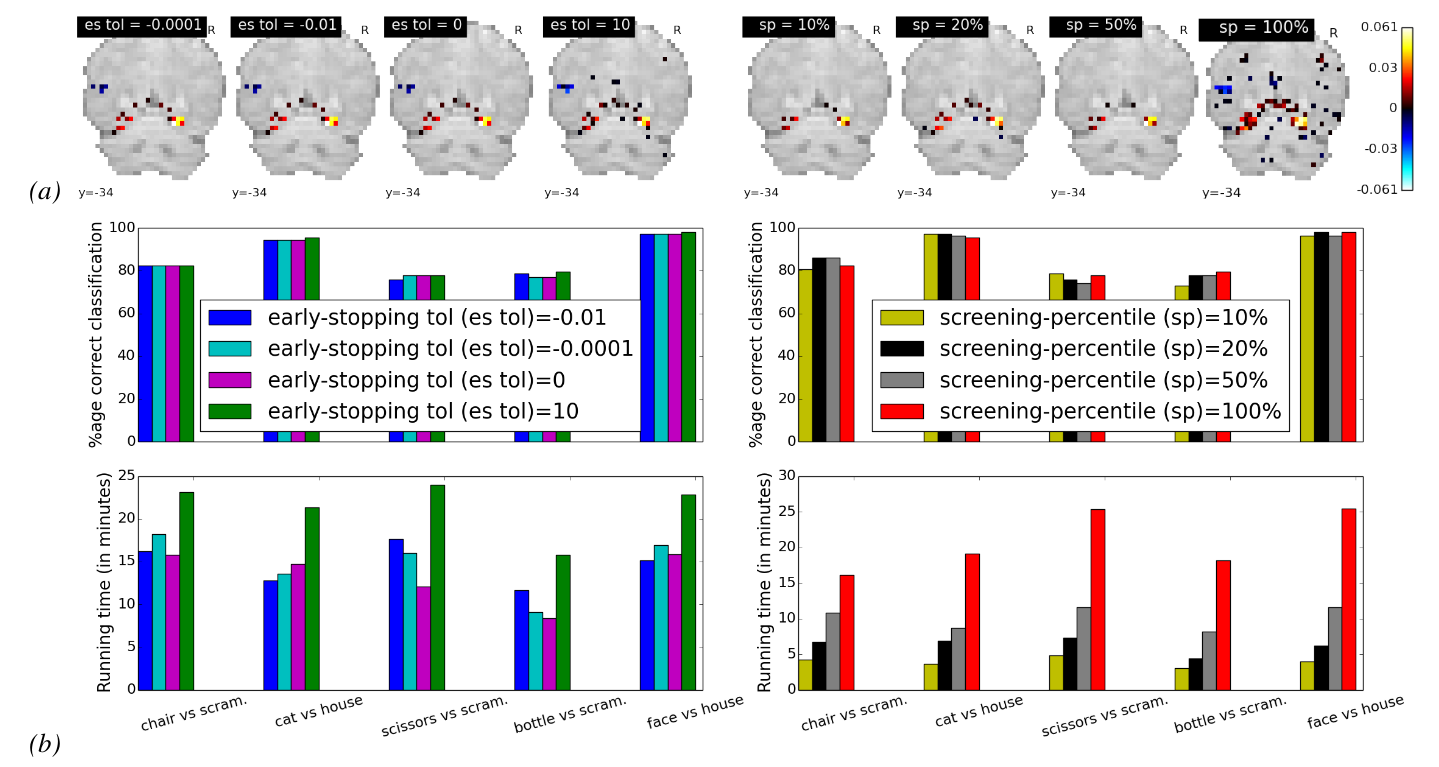
\includegraphics[width=1\linewidth]{figures/screening_weights_haxby.png}
  \caption{Predicting age from gray-matter concentration maps from the
    OASIS dataset \citep{marcus2007open}. \textbf{Top}:
    Weights maps (solutions to problem \eqref{eq:opt_pb}).
% \textbf{N.B}: The long spiky undershoots in the prediction curves
% are indicative of outliers: subjects for which spatial preprocessing
% (tissue segmentation, normalization, etc.) failed.
\textbf{Bottom-left}: Mean Square Error (MSE) in age prediction, for
different subjects of the validation set, for  varying levels of the
early-stopping tolerance (``es tol'' for short), with the
screening-percentile (sp) held constant at 100
(full-brain). \textbf{Bottom-right}: MSE in age prediction, for
varying levels of the screening-percentile (sp). \textbf{Running
  times}: Increasing \textit{est tol} (from $-10^{-4}$ to $10$): \textbf{100.2m, 171.4m, 188.8m, 289.6m}. For
increasing $sp$ ($10$ to $100$): \textbf{44.2m, 81.3m, 186.5m, 341.3m}}   
  \caption{Visual recognition dataset
    \citep{haxby2001}. \textbf{\textit{(a)}}: Weights maps
    % (maps of
    % regression coefficients $\hat{w}$)
    for the Face vs House contrast,
    for different early-stopping and univariate feature-screening
    thresholds. One can see that the supports of these maps for
    different values of the thresholds are quite similar to cases
    involving  no heuristic at all (the case where est $= 10$ and the
    where case sp $=100\%$).
    \textbf{\textit{(b)}, top-left}: Prediction scores as a function of
    the early-stopping tolerance (est), for different task contrasts.
    \textbf{\textit{(b)}, top-right}: Prediction scores as a function of
    the screening-percentile (sp), for different task contrasts.
    \textbf{\textit{(b)}, bottom-row}: Running times in minutes for the
    different thresholds of the heuristics.
    % As was to be expected, full-brain
    % (sp=100\%) is the most expensive scenario.
  }
  \label{fig:haxby}
\end{figure}
    
 In  \citep{dohmatob2015speeding}, we empirically showed on various
datasets that such screening leads to linear speed-up in the computation
time, while sacrificing prediction / classification power as long as the
screening is not very savage. We also showed that early-stopping the
estimator does not harm the accuracy of the predictions, and can also lead
to considerable (though less systematic speedups).
The result of these numerous ramblings on optimizing the SpaceNet model \eqref{eq:opt_pb} have been implemented as part of the \textit{Nilearn} package  \citep{nilearn}.


% \newthought{We have seen} in Chapter~\ref{chap:stats_fmri} that%  encoding and decoding models take 
% as input  brain activation coefficients (also known as activation patterns or beta-maps). These are usually computed by means of the general linear model (GLM), which
% relies on a \mbox{data-independent} \emph{canonical} form of the hemodynamic response function
% (HRF).


% In this chapter we describe a novel method for the simultaneous estimation of HRF and activation coefficients based on low-rank modeling, forcing the estimated HRF to be equal across events or experimental conditions,
%  yet permitting it to differ across voxels. The estimation of this model leads to
% an optimization problem that we propose to solve with using a
% \mbox{quasi-Newton} method, exploiting fast gradient computations. 
% We compare 10 different HRF modeling methods in terms of encoding and decoding
% score on two different datasets. These results show that the \mbox{R1-GLM} model
% outperforms competing methods in both encoding and decoding
% settings, positioning it as an attractive method both from the points of view
% of accuracy and computational efficiency.

% \hspace{20pt}
% \begin{shaded}
% The contributions developed in this chapter have been published in:
% \begin{itemize}
% \item F. Pedregosa, M. Eickenberg, P. Ciuciu, and B. Thirion, \emph{``Data-driven HRF estimation for encoding and decoding models''} NeuroImage, Volume 104, 1 January 2015, Pages 209-220.

% \item F. Pedregosa, M. Eickenberg, B. Thirion, and A. Gramfort, \emph{“HRF estimation improves sensitivity of fMRI encoding and decoding models”} Proc. 3nd Int. Work. Pattern Recognit. NeuroImaging, 2013.
% \end{itemize}
% \end{shaded}

% \newpage
% \vspace*{\fill}
% \minitoc
% \vspace*{\fill}
% \newpage


% \section{Sparsity and smoothness priors for improved estimation in high dimensions}
% \newthought{Michel et al. 2011, Baldasarre et al. 2012, Gramfort et al. 2013, Abraham et al. 2013, Dohmatob et al. 2014(5), Varoquaux et al. 2016}, ...

% \begin{marginfigure}[4cm]
% \hspace{-20pt}\includegraphics[width=1.2\linewidth]{chapter_3/hrfs_age.pdf}
% \caption{
% 	The HRF can vary substantially between subjects, brain regions and age. In \citept{colonnese2007development}, the authors studied the evolution of the HRF across age in rats. By comparing fMRI measurements with electrophysiological recordings, they observed two significant trends as age increased: growing amplitude and decreasing time to peak. In the figure, estimated HRF for three groups of rats (with age P13-15 < P20-30< Adult). Source: \citepp{colonnese2007development}. A comparison of the HRF in human subjects was performed in~\citepp{badillo2014multi}.
% }
% \end{marginfigure}


% fMRI acquisitions consist of successive brain scans, given in intervals ranging from 1 to 4 seconds. The extraction of time-independent \gls{activation coefficient} from the BOLD time course is commonly done with a model known as Linear General Model
% (GLM)~\citepp{Friston1995}. While
% this approach has been successfully used in a wide range of studies, it does
% suffer from limitations~\citepp{Poline2012}. For instance, the GLM commonly
% relies on a \mbox{data-independent} \emph{reference} form of the hemodynamic response function
% (HRF) to estimate the activation coefficient (also known as \emph{canonical HRF}). However it is
% known~\citepp{Handwerker2004,Badillo2013} that the shape of this response function
% can vary substantially across subjects, age and brain regions. This suggests that an adaptive modeling of this
%  response function should improve the accuracy of subsequent analysis.

% % \emph{feature-extraction} model that extracts 

% % In this section we describe a method that allows to estimate time-independent \gls{activation coefficient} given the BOLD time course. {\blue Feature extraction}. This model is known as the \emph{general linear model}~\citepp{Friston1995}. In this chapter we describe the main assumptions behind this model: a known form of the hemodynamic response function and the linear-time-invariant property between the BOLD signal and the neural response. 

% % We have seen in Chapter 2 that both encoding and decoding models take as input voxel-wise activation coefficients. These are commonly are computed by means of the General Linear Model
% % (GLM)~\citepp{Friston1995}. While
% % this approach has been successfully used in a wide range of studies, it does
% % suffer from limitations~\citepp{Poline2012}. For instance, the GLM commonly
% % relies on a \mbox{data-independent} \emph{reference} form of the hemodynamic response function
% % (HRF) to estimate the activation coefficient (also known as \emph{canonical HRF}). However it is
% % known~\citepp{Handwerker2004,Badillo2013} that the shape of this response function
% % can vary substantially across subjects, age and brain regions. This suggests that an adaptive modeling of this
% %  response function should improve the accuracy of subsequent analysis.

% To overcome the aforementioned limitation, Finite Impulse Response (FIR) models have been
% proposed within the GLM framework~\citepp{Dale1999,Glover1999}.
% These models do not assume any particular shape for the HRF and amount to
% estimating a large number of parameters in order to identify it. 
% While the FIR-based modeling makes it possible to estimate the
% activation coefficient and the HRF simultaneously, the increased flexibility
% has a cost. The estimator is less robust and prone to overfitting, i.e. to generalize poorly to unseen data. 
% In general, FIR
% models are most appropriate for studies focused on the characterization of the
% shape of the hemodynamic response, and not for studies that are primarily
% focused on detecting activation~\citep[Chapter~5]{Poldrack}.

% Several strategies aiming at reducing the number of degrees of freedom of the
% FIR model - and thus at limiting the risk of overfitting - have been proposed.
% One possibility is to constrain the shape of the HRF to be a linear
% combination of a small number of basis functions. A common choice of basis is 
% formed by three elements consisting of a reference HRF as well as its time and dispersion
% derivatives~\citepp{friston1998nonlinear}, although it is also possible to compute a
% basis set that spans a desired function
% space~\citepp{Woolrich2004}. More generally, one can also define a parametric
% model of the HRF and estimate the parameters that best fit this
% function~\citepp{Lindquist2007}. However, in this case the estimated HRF may no longer be a linear function of the input parameters. 

% Sensitivity to noise and overfitting can also be reduced through
% regularization. For example, temporal regularization has been used in the
% smooth FIR ~\citepp{Goutte2000,Ciuciu2003,Casanova2008} to favor solutions with
% small second order time derivative. These approaches require the setting of
% one or several hyperparameters, at the voxel or potentially at the parcel
% level (if several voxels in a pre-defined parcel are assumed to share some aspects of the HRF time course). Even if efficient techniques such as generalized   
% \mbox{cross-validation}~\citepp{golub1979generalized} can be used to choose the
% regularization parameters, these methods are inherently more costly than 
% \mbox{basis-constrained} methods. \mbox{Basis-constrained} methods also require
% setting the number of basis elements; however, this parameter is not
% continuous (as in the case of regularized methods), and in practice only few
% values are explored: for example the 3-element basis set formed by a reference HRF
% plus derivatives and the FIR model.  This paper focuses on basis-constrained
% regularization of the HRF to avoid dealing with hyperparameter selection with
% the goal of remaining computationally attractive.  A different approach to
% increase robustness of the estimates consists in linking the estimated HRFs
% across a predefined brain parcel, taking advantage of the spatially dependent nature of
% fMRI~\citepp{Wang2013}. However, \mbox{hemodynamically-informed}
% parcellations~\citepp{Chaari2012,Badillo2013a} rely on the computation of 
% a large number of estimations at the voxel or \mbox{sub-parcel} level.
% In this setting, the development of voxel-wise estimation procedures is complementary to the
% development of parcellation methods in that more robust estimation
% methods at the voxel level would naturally translate into more 
% robust parcellation methods. In this thesis we focus on voxel-wise
% estimation methods.


% \paragraph{Contribution}

% In this chapter we have described a method for the simultaneous estimation of HRF and activation coefficients based on low-rank modeling. While the assumptions of this model are not novel (cf.~\citepp{Makni2008,vincent2010spatially,Degras2014}), the formulation of this model as a least squares problem with a rank-one constraint is a novel contribution. This formulation allows to efficiently solve the problem using gradient-based methods.
% Finally, we evaluate the proposed model on three publicly available datasets. 

% % {\blue With respect to the work published in ~\citepp{Pedregosa2015209}, we have included in this chapter the results on a new datasets and examined the gain obtained by this model across different regions of the brain}.

\section{A small result on the rate of convergence of the ADMM algorithm}

\newthought{In our ICASSP 2016 paper} \citep{dohmatob2015local}, we studied the convergence of
the ADMM (Alternating Direction Method of
Multipliers) algorithm on a broad range of penalized regression
problems including the Lasso, Group-Lasso and Graph-Lasso,(isotropic)
TV-L1, Sparse Variation, and others, that can be written in the form

\begin{equation}
  \underset{(\w,\z) \in \mathbb{R}^p \times
    \mathbb{R}^q}{\text{minimize}}\text{ }\frac{1}{2}\|\X\w-\y\|^2 +
  \lambda\Omega(\z) \text{ subject to }\K\w
    - \z = 0,
  \label{eq:main_pb}
\end{equation}
where $\X \in \mathbb{R}^{n \times  p}$ is the design matrix; $\y \in
\mathbb{R}^n$ is a vector of measurements or classification targets; 
$\K\in\mathbb{R}^{q \times p}$ is linear operator;  $\lambda > 0$ is the
regularization parameter;
and $\Omega: \mathbb{R}^p \rightarrow (-\infty, +\infty]$ is
    the penalty, which is assumed to be a \textit{closed proper
      convex} function.
    In signal processing literature, such a problem is referred to as synthesis problem: the penalty $\Omega$ is imposed not directly on the image, but on a the output of a dictionary, $\z = \K\w$. $\K$ is referred to the analysis operator. The case $\K = \Id$ corresponds to the \textit{synthesis} setting.

\begin{marginfigure}[4cm]
  \label{fig:rates}  
  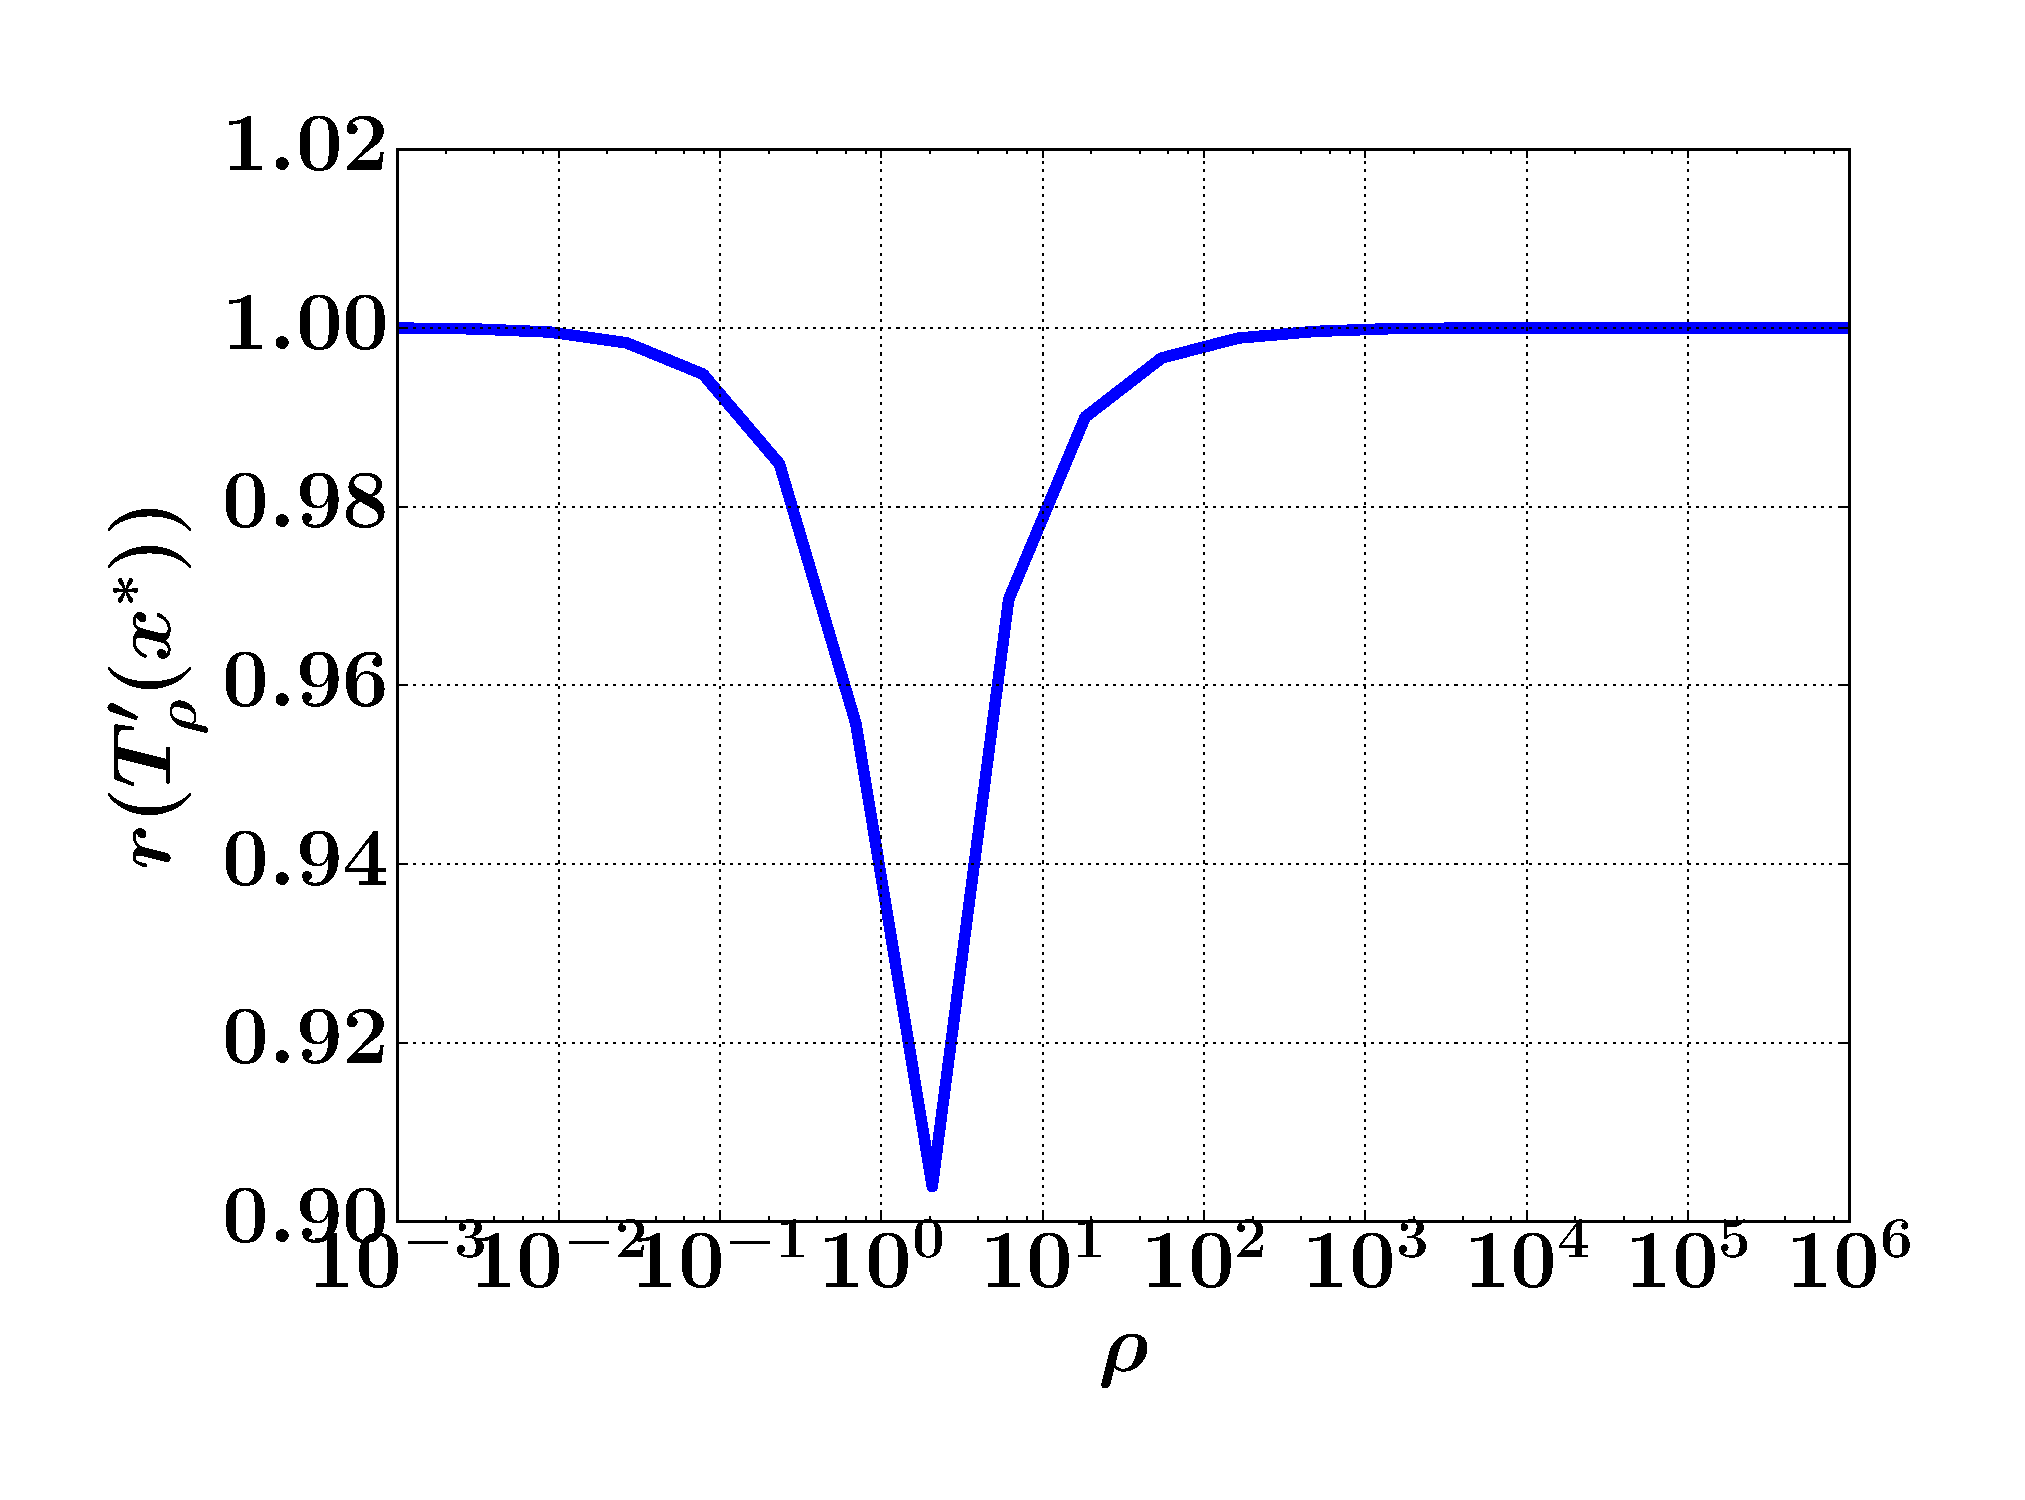
\includegraphics[width=1\linewidth]{figures/lasso_rates.pdf}%
\caption{Rate of convergence $r(\Lambda'_\rho(\x^*))$ as a function of $\rho$
  for a Lasso problem with column-rank deficient design
  matrix $\X$. Taking $\rho$ too small leads
  to badly conditioned problem (as  $\Id + (1/\rho)\X^T\X$ is then almost
  singular), and thus a slow rate of convergence (near 1). On the
  other hand, the figure suggests that taking $\rho$ ``too large''
  is also detrimental. Most remarkable, one notices that the basin of
  ``good'' $\rho$ values is rather tight, and so care must be taken in
  choosing the $\rho$ parameter.
}
\end{marginfigure} %-----------------------------------------------------------
    
First, we established a
fixed-point iteration for a nonlinear operator $\Lambda$ %\eqref{eq:factorize}
    
  \begin{eqnarray}
    \begin{aligned}
      %% Q := \X^T\X \in \mathbb{R}^{p \times p},\hspace{.5em}\Delta :=
      %% \K^T\K \in \mathbb{R}^{p \times p},\hspace{.5em}
      &\G_{\rho} :=
      \K(\K^T\K + \rho^{-1}\X^T\X)^{-1}\K^T,\hspace{.5em}
      \A_{\rho}:=[\G_{\rho}\hspace{.5em}\Id-\G_{\rho}],\\
      &\b_{\rho} := \rho^{-1}\K(\K^T\K +
      \rho^{-1}\X^T\X)^{-1}\X^T\y,\hspace{.2em}\tilde{\A}_{\rho} :=
      \A_{\rho}(.) +  \b_{\rho},\\
      &\Lambda_{\rho} :=
        \left(\prox_{(\lambda/\rho)\Omega}\circ\tilde{\A}_{\rho},
        (\Id-\prox_{(\lambda/\rho)\Omega})\circ\tilde{\A}_{\rho}\right)\\
        &(\z^{(n+1)}, \u^{(n+1)}) \leftarrow
        \Lambda_{\rho}(\z^{(n)}, \u^{(n)}),
    \end{aligned}
    \label{eq:factorize}
  \end{eqnarray}
which is equivalent to the ADMM iterates
\begin{eqnarray}
    \begin{split}
      \w^{(n+1)} &\leftarrow
      \underset{\w \in \mathbb R^p}{\argmin}\text{ }\mathcal{L}_{\rho}(\w, \z^{(n)},
      \u^{(n)}) \\
      &= (\rho \K^T\K + \X^T\X)^{-1}(\rho\K^T(\z^{(n)} -
      \u^{(n)}) + \X^T\y)\\
      \z^{(n+1)} &\leftarrow \underset{z \in \mathbb R^q}{\argmin}\text{ }\mathcal{L}_{\rho}(\w^{(n+1)},\z, \u^{(n)}) =
      \prox_{(\lambda/\rho)\Omega}(\K\w^{(n+1)} + \u^{(n)})\\
      \u^{(n+1)} &\leftarrow \u^{(n)} + \K\w^{(n+1)} -\z^{(n+1)}.
    \end{split}
\label{eq:admm}
\end{eqnarray}
We then showed that this nonlinear operator is
Fr\'echet-differentiable almost everywhere and that around each fixed
point, Q-linear convergence is guaranteed, provided the spectral
radius of the Jacobian of the operator at the fixed point is less than
1 (a classical result on stability). Moreover, this spectral radius is
then a rate of convergence for the ADMM algorithm. Also, we showed that
the support of the split variable can be identified after finitely
many iterations. In the anisotropic cases, we show that for
sufficiently large values of the tuning parameter, we recover the
optimal rates in terms of Friedrichs angles, that have appeared
recently in the literature.

\paragraph{Main theorem.} Our main results are summarized in Theorem 1 of the aforementioned paper, which we now state.
\begin{theorem} Consider the ADMM algorithm \eqref{eq:admm} on problem
  \eqref{eq:main_pb}, where $\Omega$ is an $\ell_{2,1}$ mixed-norm on
  $d \ge 1$ blocks each of size $c \ge 1$, for a total of $q = d
  \times c$ features. Let the operators $\B{A}$, $\tilde{\B{A}}$, and $\Lambda$ be
  defined as defined above, with the $\rho$ subscript
  dropped for ease of notation. Let For $\B{x} = (\B{z}, \B{u}) \in\mathbb{R}^{q+q}$, let $\Lambda_1(\B{x}) \in \mathbb R^q$ denote the first $q$ coordinates of $\Lambda(\B{x})$, i.e its $z$-part. Define
  \begin{itemize}
    \item $\supp(\B{z}) := \{j\in[d]\text{ }|\text{ }z_{j:j+c-1} \ne
      0\}$;
      \item $\mathcal{A}_1(\B{z}) := \{\B{z}' \in \mathbb{R}^{q} |
    \supp(\B{z}') = \supp(\B{z})\}$, and $\mathcal A(\B{x}) := \mathcal A_1(\B{z}) \oplus \mathbb R^q$;
   \item $\tilde{\B{x}} := (\tilde{\B{x}}_j)_{j \in [d]} := \tilde{\A}\B{x}$, $\kappa :=
    \lambda / \rho$, $\epsilon(\B{x}) :=
      \underset{j \in [d]}{\min}\text{}|\|\tilde{\B{x}}_j\|-\kappa| \ge 0$.
    \end{itemize}
Then the following hold:
\begin{itemize}
\item[\textit{(a)}] \textbf{Attractivity of supports.} For all $\B{x} \in
  \mathbb{R}^{q+q}$, we have
  \[\Lambda(\bar{\mathbb{B}}_{2q}(\B{x},\epsilon(\B{x})/\|\A\|)) \subseteq
  \bar{\mathbb{B}}_{2q}(\Lambda(\B{x}),\epsilon(\B{x})) \cap
  \mathcal{A}(\Lambda(\B{x})).\] In
  particular, if $\B{x}^*$ is a fixed-point of $\Gamma$, then
  \[
  \Lambda(\bar{\mathbb{B}}_{2q}(\B{x}^*,\epsilon(\B{x}^*)/\|\A\|))
  \subseteq
  \bar{\mathbb{B}}_{2q}(\B{x}^*,\epsilon(\B{x}^*)) \cap \mathcal{A}(\B{x}^*).
  \]
\item[\textit{(b)}] \textbf{Fr\'echet-differentiability.} If $\B{x} \in
  \mathbb{R}^{q+q}$ with
  $\epsilon(\B{x}) > 0$, then $\Lambda$ is Fr\'echet-differentiable at $\B{x}$ with
  derivative
\begin{eqnarray}
  \Lambda'(\B{x}) = \B{F}_{\B{x}}\A \in \mathbb{R}^{2q \times 2q},
\label{eq:linear}
\end{eqnarray}
where $\B{F}_{\B{x}} := [\B{D}_{\B{x}} \hspace{.6em} \Id - \B{D}_{\B{x}}]^T$ and  $\B{D}_{\B{x}} \in
\mathbb{R}^{q \times q}$ is a block-diagonal matrix
with block $\B{D}_{\B{x},j} \in \mathbb{R}^{c \times c}$
given by
\begin{eqnarray}
\B{D}_{\B{x},j} = \begin{cases}\Id -
  \frac{\kappa}{\|\tilde{\B{x}}_j\|}P_{\langle
        \tilde{\B{x}}_j \rangle^\perp}, &\mbox{ if } j \in
  \supp(\Lambda_1(\B{x})),\\ 0, &\mbox{ otherwise.}\end{cases}
\label{eq:d}
\end{eqnarray}
In particular,  when $c=1$,  each $\B{D}_{\B{x}^,j}$ reduces to a
bit $\in \{0,1\}$ which indicates whether the $j$th feature is
active, and $\B{D}_{\B{x}}$ reduces to a diagonal projector matrix with only
0s and 1s.

\item[\textit{(c)}] Let $\B{x}^* = (\B{z}^*, \B{u}^*)\in \mathbb{R}^{q+q}$ be any fixed-point of $\Gamma$.
\begin{itemize}
\item[\textit{(1)}] \textbf{Finite-time identification of
    active set.} If the closed ball $\bar{\mathbb{B}}_{2q}(\B{x}^*, \epsilon(\B{x}^*)/\|\A\|)$
    contains any point of the sequence of iterates $x^{(n)}$, then the
    active set $\mathcal{A}(\B{x}^*)$ is
    identified after finitely many iterations, i.e
    \begin{eqnarray}
      \label{eq:id}
      \exists N_{\B{x}^*} \ge 0 \text{ s.t }\B{x}^{(n)} \in \mathcal{A}(\B{x}^*)
      \forall n \ge N_{\B{x}^*}.
    \end{eqnarray}
      In particular, \eqref{eq:id} holds if $\B{x}^{(n)}$ converges to $\B{x}^*$.

\item[\textit{(2)}] \textbf{Local Q-linear convergence.}
If $\epsilon(\B{x}^*) > 0$ and $r(\Lambda'(\B{x}^*)) < 1$, then the iterates
$x^{(n)}$ converge locally Q-linearly to $\B{x}^*$
at the rate $r(\Lambda'(\B{x}^*))$.

\label{thm:frechet}
\item[\textit{(3)}] \textbf{Optimal rates in the anisotropic case.}
If $c=1$ (as in anisotropic TV deconvolution) and $\rho$ is large, then the optimal rate of convergence
rate is the cosine of the Friedrichs angle between
$\mathrm{Im}\;\K$ and $\mathrm{Im}\;\B{D}_{\B{x}^*} \simeq \mathcal A_1(\B{z}^*)$. If in addition
$K = \Id$ (as in synthesis inverse problems like the Lasso, sparse  Spike-deconvolution, etc.), then
the whole algorithm converges in finite time.
\end{itemize}
\end{itemize}
\end{theorem}

\paragraph{Experimental results.}
\begin{figure*}[!htbp]
  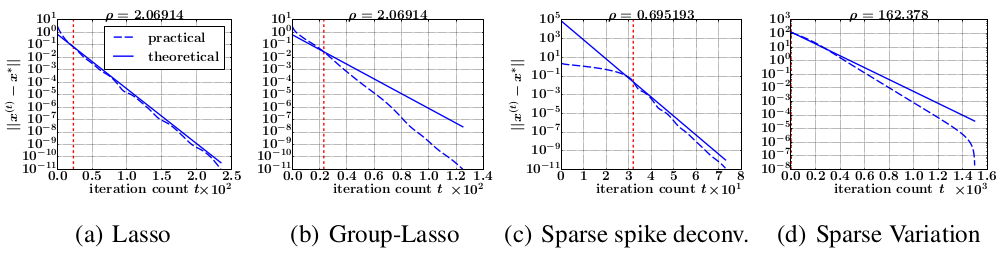
\includegraphics[width=1\linewidth]{figures/admm.png}
  \caption{{Experimental results from ICASSP paper}  \citep{dohmatob2015local}\textbf{.} showing local Q-linear convergence for ADMM
    on problem \eqref{eq:main_pb}. %% Results for
  %% all the other values of $\rho$ are provided in the supplementary matrials.
  The ``theoretical'' line is the exponential
  curve $t \mapsto \|\x^{(0)} - \x^*\|r(\Lambda'(\x^*))^t$. The red broken
  vertical line marks the instant the support the support of the fixed-point $\x^*$
  % = (\z^*,\u^*)$
  is identified.
}  
\end{figure*}
 For notation, refer to Theorem 1 of the paper.
  We can see from figure that the upper bound for the local convergence
  rate is satisfied. Each shown thumbnail
  is for the value of $\rho$ for
  which the spectral radius $r(\Lambda_\rho'(\B{x}^*))$ was smallest.
  


% \section{Generalized online dictionary learning: richer penalties on the components}
% \newthought{In our NIPS 2017 paper} \citep{dohmatob2016},




% The reference HRF models a general response function that has been proven successful under a wide range of circumstances. However, a number of studies have shown that the shape of the hemodynamic response differ substantially among subjects~\citepp{Aguirre1998360} and brain regions~\citepp{Schacter1997259}. One popular approach to model small offsets in the time to peak and dispersion is to consider that the HRF is modeled from a basis set consisting of the reference HRF plus its derivative with respect to time and dispersion (see Figure~\ref{fig:hrf_basis}). The rationale for considering this basis set comes from the fact that it corresponds to the first-order approximation to the Taylor expansion of the reference HRF. Given the reference HRF, $h(t)$, a time-shifted version of the hemodynamic response can be described as $h(t + \delta)$. A Taylor series expansion of $h(t + \delta)$ with respect to $\delta$ gives the approximation $h(t) + \delta h'(t) + \ldots$~, implying that small offsets can be modeled by considering a linear combination of the reference HRF plus its time derivative. In similar fashion we can model small perturbations in dispersion (the width of the response) by considering the reference HRF plus its dispersion derivative. 


% \begin{figure*}
% \includegraphics[width=.5\linewidth]{figures/chapter_1/canonical_hrf_basis.pdf}
% \includegraphics[width=.5\linewidth]{figures/chapter_1/canonical_hrf_generated.pdf}
% \caption{A popular basis set to generate a family of HRF functions is the ``reference HRF plus derivatives''. In the left plot, we show a reference HRF together with its time and dispersion derivatives. This basis set can model small variations in temporal shifts and dispersion with respect to the reference HRF. In the right plot we show a sample set of HRFs generated by this basis. The weights of these response functions are Gaussian random vectors centered around the reference HRF.}\label{fig:hrf_basis} 
% \end{figure*}

% A popular example of basis set is presented in Figure~\ref{fig:hrf_basis} and consists of the reference HRF plus its time and dispersion (width) derivatives. While in the GLM with fixed HRF each regressor of the design matrix consisted of the convolution of the reference HRF with the stimulus function, in this case each regressor consist in the convolution of a basis element with the stimulus function. This results in a  design matrix of size $n \times d k$ instead of $n \times k$, where $d$ is the number of basis elements. If $d=1$ and the basis element is the reference HRF, then this setting coincides with the standard GLM. A least squares estimate of the activation coefficients $\hat{\bfbeta} = \argmin_{\bfbeta}\|\B{y} - \B{X}\bfbeta \|^2$ will result in a vector of $d$ elements for each condition. 


% The design matrix of a GLM using the basis set of the ``refence HRF plus derivatives'' is shown in Figure~\ref{fig:glm1}. The columns in this design matrix are each one of the basis elements convolved with the stimulus function for the different conditions.




% \section{Basis and rank-constrained GLM}

% In the basis-constrained GLM, the HRF estimation is performed 
% independently for each condition. This method works reliably whenever
% the number of conditions is small, but in experimental designs with a large
% number of conditions it performs poorly due to the increased variance of the estimates.
% % put ref?

% % In this model we promote a common HRF
% % across the various stimuli, which should result in more robust estimates~\citepp{Makni2008,vincent2010spatially}.
% In this work we consider a model in which a common HRF is shared
% across the different stimuli. Besides the estimation of the HRF,
% a unique coefficient is obtained per column of our event
% matrix. This amounts to the estimation of $k + d$ free parameters
% instead of $k \times d$ as in the standard basis-constrained GLM setting.

% The novelty of our method stems from the observation that the formulation of the GLM with a
% common HRF across conditions translates to a rank constraint on the vector of estimates. 
% This assumption amounts to enforcing the vector of
% estimates to be of the form $\bfbeta_{\B{B}} = [\mathbf{h} {\beta}_1, \mathbf{h} \beta_2, \cdots, \mathbf{h}
% \beta_k]$ for some HRF $\mathbf{h} \in \RR^d$ and a vector of coefficients $\bfbeta \in \RR^k$. More compactly, this can be written as $\bfbeta_{\B{B}} = \vecop(\B{h}
% \bfbeta^T)$. This can be
% seen as a constraint on the vector of coefficients to be the vectorization of a rank-one
% matrix, hence the name {\it Rank-1 GLM (R1-GLM)}.


% \begin{figure*}[t]
% \centering \includegraphics[width=0.8\linewidth]{figures/chapter_1/glm_3hrf.pdf}
% \caption{A basis-constrained GLM design matrix. The basis set consists of the reference HRF plus its time and dispersion derivative. As in the GLM introduced in Chapter~\ref{chap:intro_fmri} (Fig.~\ref{fig:glm1}), each column is the convolution of one basis function with the stimulus function. Here, the usage of 3 basis functions (instead of one) results in a design matrix with $3 k$ regressors}\label{fig:glm_3hrf}
% \end{figure*}


% In this model, the coefficients have no longer a closed form expression,
% but can be estimated by minimizing the following loss function. Given $\B{X}_{\B{B}}$ and $\B{y}$ as before, $\B{Z} \in \RR^{n \times q}$ a matrix of nuisance parameters such as drift regressors, we define $F_{\text{R1}}(\B{h}, \bfbeta, \bfomega, \B{X}_{\B{B}}, \B{y}, \B{Z}) = \frac{1}{2}\|\mathbf{y} - \mathbf{X}_{\B{B}} \vecop(\B{h} \bfbeta^T) - \B{Z} {\bfomega}\| ^2$ to be the objective function to be minimized. The optimization problem reads:
% %
% \begin{eqnarray}
% \label{eq:r1}
% \begin{aligned}
% \hat{\B{h}}, ~\hat{\bfbeta},~ \hat{\bfomega} ~=~& \argmin_{\B{h}, \bfbeta, {\bfomega}} ~ F_{\text{R1}}(\B{h}, \bfbeta, \bfomega, \B{X}_{\B{B}}, \B{y}, \B{Z})\\
% &\text{subject to } \|\B{B} \B{h}\|_{\infty} = 1 \text{ and } \langle \B{B} \B{h}, \B{h}_{\text{ref}}\rangle > 0 \enspace ,
% \end{aligned}
% \end{eqnarray}
% %
% The norm constraint is added to avoid the scale ambiguity between $\B{h}$ and $\bfbeta$
% and the sign is chosen so that the estimated HRF correlates
% positively with a given reference HRF $\B{h}_{\text{ref}}$.
% Otherwise the signs of the HRF and $\bfbeta$ can be simultaneously flipped without changing
% the value of the cost function. Within its feasible set, the optimization problem
% is {\it smooth} and is convex with respect to $\B{h}$, $\bfbeta$ and $\bfomega$,
%  however it is not {\it jointly convex} in variables $\B{h}$, $\bfbeta$ and $\bfomega$.

% From a practical point of view this formulation has a number of advantages.
% First, in contrast with the GLM without rank-1 constraint the estimated
% coefficients are already factored into the estimated HRF and the activation
% coefficients. That is, once the estimation of the model parameters
% from Eq.~\eqref{eq:r1} is obtained, $\hat{\bfbeta}$ is a vector of size $k$ and $\hat{\B{h}}$ is a
% vector of size $d$ that can be both used in subsequent analysis, while in models
% without rank-1 constraint only the vector of coefficients (equivalent to 
% $\text{vec}(\B{h} \bfbeta^T)$ in rank-1 constrained models) of size $k
% \times d$ is estimated. In the latter case, the estimated HRF and the beta-maps
% still have to be extracted from this vector by methods such as normalization by the peak of the HRF,
% averaging or projecting to the set of Rank-1 matrices.

% Second, it is readily adapted to prediction on unseen trials. While for
% classical (non rank-1 models) the HRF estimation is performed per condition with no HRF associated with unseen conditions, in this setting, because the
% estimated HRF is linked and equal across conditions it is natural to use this
% estimate on unseen conditions. This setting occurs often in encoding models 
% where prediction on unseen trials is part of the cross-validation procedure.

% This model can also be extended to a parametric HRF model. That is,
% given the hemodynamic response defined as a function $h: \RR^{d_1} \to \RR^d$ of some parameters
% $\bfalpha$, we can formulate the analogous model of Eq.~\eqref{eq:r1} as an
% optimization over the parameters $\bfalpha$ and $\bfbeta$ with the design matrix
% $\B{X}_{\text{FIR}}$ given by the convolution of the event matrix with the FIR basis:
% %
% \begin{eqnarray}
% \label{eq:r1_parametric}
% \begin{aligned}
% \hat{\bfalpha}, ~\hat{\bfbeta}, ~\hat{\bfomega} ~=~&\argmin_{\bfalpha, \bfbeta, \bfomega} 
% F_{\text{R1}}(h(\bfalpha), \bfbeta, \bfomega, \B{X}_{\text{FIR}}, \B{y}, \B{Z}) \\
% &\text{subject to } \| h(\bfalpha)\|_{\infty} = 1  \text{ and } \langle h(\bfalpha), \B{h}_{\text{ref}} \rangle > 0
% \end{aligned}
% \end{eqnarray}

% In section \ref{sub:optim} we will discuss optimization strategies for both
% models.

% % \section{Alternative formulations}

% % We present two alternative formulations

% \section{Extension to separate designs}

% \begin{marginfigure}[8cm]
% \center \includegraphics[width=.6\linewidth]{chapter_3/ls-s.pdf}
% \caption{In the GLM with separate designs model of~\citept{Mumford2012}, the design matrix contains two regressors. The first one is the
% regressor associated with a given condition and the second one is the sum of all
% other regressors. Source: \citepp{Turner2012}}
% \end{marginfigure}

% An extension to the classical GLM that improves the estimation with correlated
% designs was proposed in~\citepp{Mumford2012}.
% In this setting, each voxel is modeled as a linear combination of two
% regressors in a design matrix $\B{X}_\text{GLM}$. The first one is the
% regressor associated with a given condition and the second one is the sum of all
% other regressors. This results in $k$ design matrices, one for each condition.
% The estimate for a given condition is given by the first element in the two-dimensional
% array ${\B{X}_{\text{S}i}}^{\dagger} \B{y}$, 
% where $\B{X}_{\text{S}i}$ is the design matrix for
% condition $i$. We will 
% denote this model GLM with separate designs (GLMS). It has been reported to find
% a better estimate in rapid event designs leading to a boost in accuracy for
% decoding tasks~\citepp{Mumford2012, Schoenmakers2013, Lei2013}.

% This approach was further extended in~\citepp{Turner2012} to
% include FIR basis instead of the predefined canonical function. Here we employ it 
% in the more general setting of a  
% predefined basis set. Given a set of basis
% functions we construct the design matrix for condition $i$ as the columnwise
% concatenation of two matrices $\B{X}^0_{\text{BS}i}$ and $\B{X}^1_{\text{BS}i}$.
% $\B{X}^0_{\text{BS}i}$ is given by the columns associated
% with the current condition in the GLM matrix and $\B{X}^1_{\text{BS}i}$ is
% the sum of all other columns.
% In this case, the vector of estimates is given by the first $d$ vectors of
% $\B{X}_{\text{BS}i}^{\dagger} \B{y}$. See~\citepp{Turner2012} for a more complete description of the matrices $\B{X}^0_{\text{BS}i}$ and $\B{X}^1_{\text{BS}i}$.

% It is possible to use the same rank-1
% constraint as before in the setting of separate designs, linking the HRF 
% across conditions. We will refer to this model as \emph{Rank-1 GLM with separate designs (R1-GLMS)}. In this case the objective function has the form
% $F_{\text{R1-S}}(\B{h}, \bfbeta, \bfomega, \B{r}, \B{X}_{\B{B}}, \B{y}, \B{Z}) = \frac{1}{2}\sum_i^k \|\B{y} - \beta_i \B{X}^0_{\text{BS}i} \B{h} - r_i \B{X}^1_{\text{BS}i} \B{h} - \B{Z} \bfomega\| ^2 $, where $\B{r} \in \RR^d$ is a vector representing the activation of all events except the event of interest and 
% will not be used in subsequent analyses. We can 
% compute the vector of estimates $\hat{{\bfbeta}}$ as the solution to the optimization
% problem
% %
% \begin{eqnarray}
% \label{eq:r1_separate}
% \begin{aligned}
% \hat{\bfbeta}, ~\hat{\bfomega},~\hat{\B{h}},~\hat{\bf{r}} ~= ~&\argmin_{\B{h}, \bfbeta, \bfomega, \B{r}} F_{\text{R1-S}}(\B{h}, \bfbeta, \bfomega, \B{r}, \B{X}_{\B{B}}, \B{y}, \B{Z}) \\
% &\text{subject to } \|\B{B} \B{h}\|_{\infty} = 1 \text{ and } \langle \B{B} \B{h}, \B{h}_{\text{ref}} \rangle > 0
% \end{aligned}
% \end{eqnarray}
% %


% \section{Optimization}
% \label{sub:optim}


% For the estimation of rank-1 models on a full brain volume, a  model is estimated at each voxel separately. Since a typical brain volume contains more than 40,000 voxels, the efficiency of the estimation at a single voxel is of great importance. In this section we will detail an efficient procedure based on quasi-Newton methods for the estimation of R1-GLM and R1-GLMS models on a given voxel.


% One approach to minimize \eqref{eq:r1} is to alternate the minimization
% with respect to the variables $\bfbeta$, $\B{h}$ and $\bfomega$. By recalling the Kronecker product identities~\citep[Chapter 4.3]{horn1991topics}, and using the identity \(\vecop(\B{h}\bfbeta^T) = \bfbeta\otimes \B{h}\)
% we can rewrite the objective function~\eqref{eq:r1} to be minimized as:
% %
% \begin{gather}
% \label{eq:kron}
% \frac{1}{2}\|\B{y} - \B{X}_{\B{B}} (\bfbeta \otimes \B{h}) - \B{Z} \bfomega\| ^2 = \\ \frac{1}{2}\|\B{y} - \B{X}_{\B{B}} (\B{I} \otimes \B{h}) \bfbeta - \B{Z} \bfomega\| ^2 = \\ \frac{1}{2}\|\B{y} - \B{X}_{\B{B}} (\bfbeta \otimes \B{I}) \B{h} - \B{Z} \bfomega\|^2 \enspace.
% \end{gather}
% %
% Updating $\B{h}$, $\bfbeta$ or $\bfomega$ sequentially thus amounts to solving a (constrained) least squares
% problem at each iteration. A similar procedure is detailed in~\citepp{Degras2014}. However, this approach requires computing the
% matrices $\B{X}_{\B{B}} (\bfbeta \otimes \B{I})$ and $\B{X}_{\B{B}} (\B{I} \otimes \B{h})$ at each iteration, which are typically dense,
% resulting in a high computational cost per iteration. Note also that the optimization problem is not jointly convex in variables $\B{h}, \bfbeta, \bfomega$, therefore we cannot apply convergence guarantees from convex analysis.

% We rather propose a more efficient approach by optimizing both variables jointly. We define a 
% global variable $\B{z}$ as the concatenation of $(\B{h}, \bfbeta, \bfomega)$ into a single vector, $\B{z} = \vecop([\B{h}, \bfbeta, \bfomega])$,
%  and cast the problem as an optimization with respect to this new variable.
% Generic solvers for numerical
% optimization~\citepp{nocedal2006numerical} can then be used. The solvers that we will consider take as
% input an objective function and its gradient. In this case, the partial derivatives with respect to variable $\B{z}$ can be written as 
% $\partial F_{\text{R1}} / \partial \B{z} = \vecop([\partial F_{\text{R1}} / \partial \B{h}, \partial F_{\text{R1}} / \partial{\bfbeta}, \partial F_{\text{R1}} / \partial {\bfomega}])$, whose expression can be
% easily derived using the aforementioned Kronecker product identities:
% %
% \begin{equation*}
%     \left\{
%     \begin{aligned}
%         \frac{\partial F_{\text{R1}}}{\partial \B{h}}=& - (\bfbeta^T \otimes \B{I}) \B{X}^T (\B{y} - \B{X} \vecop(\B{h} \bfbeta^T) - \B{Z} \bfomega) \\
%         \frac{\partial F_{\text{R1}}}{\partial \bfbeta}=& - (\B{I} \otimes \B{h}^T) \B{X}^T (\B{y} - \B{X} \vecop(\B{h} \bfbeta^T) - \B{Z} \bfomega) \\
%         \frac{\partial F_{\text{R1}}}{\partial \bfomega}=& - \B{Z}^T (\B{y} - \B{X} \vecop(\B{h} \bfbeta^T) - \B{Z} \bfomega)
%     \end{aligned}
%     \right.
% \end{equation*}



% If instead a parametric model of the HRF is used as in Eq.~\eqref{eq:r1_parametric}, the equivalent partial derivatives can be easily computed by the chain rule.


% For the sake of efficiency, it is essential to avoid evaluating the Kronecker products naively,
%  but rather reformulate them using the above mentioned Kronecker identities. For example, the matrix $\B{M} = \B{X} (\B{I} \otimes \B{h})$ should not be computed explicitly but should rather be stored as a linear operator such that when applied to a vector $\B{a} \in \RR^k$ it computes $M(\B{a}) = \B{X} (\B{a} \otimes \B{h})$, avoiding thus the explicit computation of $\B{I} \otimes \bfbeta$. 


% Similar equations can be derived for the rank-1 model with separate designs of Eq.~\eqref{eq:r1_separate} (\mbox{R1-GLMS}), in which
% case the variable $\B{z}$ is defined as the concatenation of $(\B{h}, \bfbeta, \bfomega, \B{r})$, i.e. $\B{z} = \vecop([\B{h}, \bfbeta, \bfomega, \B{r}])$. The gradient of $F_{\text{R1-S}}$ with respect to $\B{z}$ can be computed as $\partial F_{\text{R1-S}} / \partial \B{z}$ = $\vecop([\partial F_{\text{R1-S}} / \partial \B{h},$ $\partial F_{\text{R1-S}} / \partial{\bfbeta}, \partial F_{\text{R1-S}} / \partial {\bfomega}, F_{\text{R1-S}} / \partial {\B{r}}])$. The partial derivatives read:
% %
% \begin{equation*}
%     \left\{
%     \begin{array}{lcl}
%         \frac{\partial F}{\partial \B{h}} &=& \sum_i^k - (\B{X}^0_{\text{BS}_i}\bfbeta_i - \B{X}^1_{\text{BS}_i} r_i)^T (\B{y} - \bfbeta_i \B{X}^0_{\text{BS}_i} h - w_i \B{X}^1_{\text{BS}_i} \B{h}) \\
%         \frac{\partial F}{\partial \beta_i} &=& -(\B{X}^0_{\text{BS}_i} \B{h})^T (\B{y} - \bfbeta_i \B{X}^0_{\text{BS}_i} \B{h} - w_i \B{X}^1_{\text{BS}_i} \B{h}) \\
%         \frac{\partial F}{\partial \omega_i} &=& -\B{Z}^T (\B{y} - \bfbeta_i \B{X}^0_{\text{BS}_i} \B{h} - w_i \B{X}^1_{\text{BS}_i} \B{h}) \\
%         \frac{\partial F}{\partial r_i} &=& -(\B{X}^1_{\text{BS}_i} \B{h})^T (\B{y} - \bfbeta_i \B{X}^0_{\text{BS}_i} \B{h} - w_i \B{X}^1_{\text{BS}_i} \B{h}) \\
%     \end{array}
%     \right.
% \end{equation*}

% \begin{marginfigure}
% \hspace{-10pt}\includegraphics[width=1.1\linewidth]{chapter_3/bench_r1.pdf}
% \caption{Convergence of different first-order and quasi-newton optimization algorithms for the R1-GLM model on a single voxel. ``TNC'' and ``Newton-CG'' are two different implementations of the truncated Newton~\citepp{nash1984newton} method (the first one in C and the second one in Python), ``L-BFGS-B'' is the Limited-memory BFGS algorithm with box constraints as implemented in~\citepp{zhu1997algorithm}, ``trust-ncg'' is the Newton conjugate gradient trust-region 
% algorithm and ``CG'' is the conjugate gradient algorithm, both of them described in~\citepp{nocedal2006numerical}. We found that in general the L-BFGS-B gives the best performance among these methods.}
% \end{marginfigure}

% % \todo[color=blue!60, inline]{Used an eqnarray*, because this was awfully "align*"ed. It still isn't perfect though. Maybe we need to bind the left hand sides to the left? The same theoretically goes for the equations just above}

% A good initialization plays a crucial role in the convergence of any iterative
% algorithm. We have used as initialization for the R1-GLM and R1-GLMS models the solution given by the GLM with
% separate designs (GLMS). Since the GLM with separate designs scales linearly in the number of voxels, this significantly reduces computation time whenever
% an important number of voxels is considered.

% Whenever the design matrix $\B{X}_{\B{B}}$ has more rows than columns (as is
% the case in both datasets we consider with $\B{B}$ the 3HRF basis), it is possible to
% find an orthogonal transformation that significantly speeds up the computation
% of the Rank-1 model. Let $\B{Q}, \B{R}$ be the ``thin'' QR decomposition of
% $\B{X}_{\B{B}} \in \RR^{n \times d k}$, that is, $\B{Q} \B{R} = \B{X}_{\B{B}}$ with $\B{Q}
% \in \RR^{n \times d k}$ an orthogonal matrix and $\B{R} \in \RR^{d k \times d k}$ 
% a triangular matrix. Because of the invariance of the Euclidean norm to orthogonal
% transformations, the change of variable $\B{X}_{\B{B}} \leftarrow \B{Q}^T
% \B{X}_{\B{B}}$, $\B{y} \leftarrow \B{Q}^T \B{y}$ yields a Rank-1 model in Eq.~\eqref{eq:r1}
% with equivalent solutions. This reduces the size of the design matrix to a square triangular matrix of size $d k \times d k$ (instead of $n \times d k$) and reduces the explained variable $\B{y}$ to a vector of size $k d$ (instead of $n$). After this change of variable, the convergence of the Rank-1 model is significantly faster due to the faster computation of the objective function and its partial derivatives.  We have observed that the total running time of the algorithm can be
% reduced by 30\% using this transformation.


% Some numerical solvers such as L-BFGS-B~\citepp{liu1989limited}
% require the constraints to be given as box constraints. While our original
% problem includes an equality constraint we can easily
% adapt it to use convex box constraints instead.
% We replace the equality constraint $\|\B{B h}\|_{\infty} = 1$ by
% the convex inequality constraint $\|\B{B h}\|_{\infty} \leq 1$, which is equivalent
% to the box constraint $-1 \leq (\B{B h})_i \leq 1$ supported by the above solver. 
% However, this change of constraint
% allows solutions in which $\B{h}$ can be arbitrarily close to zero. To avoid such
% degenerate cases we add the smooth term $-\|\B{B}(:, 1) h_1\|^2 _2$ to the cost function. Since
% there is a free scale parameter between $\B{h}$
% and $\bfbeta$, this does not bias the problem, but forces $\B{B h}$ to lie as far as possible from the origin (thus saturating the box constraints). Once a descent
% direction has been found by the \mbox{L-BFGS-B} method we perform a line search
% procedure to determine the step length. The line-search
% procedure was implemented to satisfy the strong Wolfe conditions~\citepp{nocedal2006numerical}.
% Finally, when the optimization algorithm has converged to a stationary point, 
% we rescale the solution setting to ensure that the equality constraint. This still leaves a sign ambiguity between the estimated HRF and the associated beta-maps. To make these parameters identifiable, the sign of the estimated HRF will be chosen so that these correlate positively with the reference HRF.

% We have compared several first-order (Conjugate Gradient), \mbox{quasi-Newton}
% (L-BFGS) and Newton methods on this problems and found that in general \mbox{quasi-Newton} methods performed best in terms of computation time. In our
% implementation, we adopt the L-BFGS-B as the default solver. 

% In Algorithm~\ref{alg1} we describe an algorithm based on L-BFGS that can be used to optimize R1-GLM and R1-GLMS models (a reference implementation for the Python language is described in subsection Software). Variable $\B{r}$ is only used for the R1-GLMS method and its use is denoted within parenthesis, i.e. $(, \B{r})$, so that for the R1-GLM it can simply be ignored.
% %
% \begin{algorithm}
% \caption{Optimization of R1-GLM and R1-GLMS models}
% \label{alg1}
% \begin{algorithmic}[1]
% \REQUIRE Given initial points $\bfbeta_0 \in \RR^k, \B{h}_0 \in \RR^d, {\bfomega}_0 \in \RR^q ~(, \mathbf{r}_0 \in \RR^k)$, convergence tolerance $\epsilon > 0$, inverse Hessian approximation $\B{H}_0$. 
% \ENSURE $\bfbeta_m, \B{h}_m$
% \STATE {(Optional)}: Compute the QR decomposition of $\B{X}_{\B{B}}$, $\B{Q} \B{R} = \B{X}_{\B{B}}$, and replace $\B{X}_{\B{B}} \leftarrow \B{Q}^T \B{X}_{\B{B}}, \B{y} \leftarrow \B{Q}^T \B{y}$
% \STATE Initialization. Set $m \leftarrow 0$, $\B{z} \leftarrow \vecop([\B{h}_0, \bfbeta_0, \bfomega_0 (, \B{r}_0)])$
% \WHILE{$\|\nabla f\| > \epsilon$}
% \STATE Compute search direction.  Set $\B{p}_m \leftarrow - \B{H}_m \nabla f(\B{h}_m, \bfbeta_m, \bfomega_m (, \B{r}_m))$
% by means of the L-BFGS algorithm.
% \STATE {Set $\B{z}_{m+1} = \B{z}_m + \gamma_m \B{p}_m$, where $\gamma_m$ is computed from a line search procedure subject to the box constraints $\|\B{h}_m\|_{\infty} \leq 1$}.
% \STATE $m \leftarrow m+1$
% \ENDWHILE 
% \STATE Extract R1-GLM(S) parameters from $\B{z}_m$. Set $\B{h}_m \leftarrow \B{z}_m(1:d), \bfbeta_m \leftarrow \B{z}_m(d+1:m+d)$
% \STATE Normalize and set sign so that the estimated HRF is positively correlated with a reference HRF: $q_m \leftarrow \|\B{h}_m\|_{\infty} \text{sign}(\B{h}_m^T \B{h}_{\text{ref}}),~ \B{h}_m \leftarrow \B{h}_m / q_m, ~\bfbeta_m \leftarrow \bfbeta_m q_m$
% \end{algorithmic} 
% \end{algorithm}

% The full estimation of the R1-GLM with 3HRF basis for one subject of the
% dataset described in section {\it Dataset 2: decoding of potential gain
% levels} ($16 \times 3$ conditions, $720$ time points, $41,622$ voxels) took 14
% minutes in a 8-cores Intel Xeon 2.67GHz machine. The total running time for
% the 17 subjects was less than four hours.


% \section{Software}

% We provide a software implementation of all the models discussed in this section
% in the freely available (BSD licensed) pure-Python package \textsf{hrf\_estimation}
% available at {\href{https://pypi.python.org/pypi/hrf\_estimation}{https://pypi.python.org/pypi/hrf\_estimation}}~. This software is further described in Section~\ref{subsec:hrf_estimation}.

% \section{Smooth Sparse Online Dictionary Learning}

% With the aim of making the results easily reproducible, we have
% chosen two freely available datasets to validate our approach and to compare
% different HRF modeling techniques.


% \section{Dataset 1: encoding of visual information}\label{subsec:encoding_dataset}

% The first dataset we will consider is 
% described in~\citepp{Kay2008,naselaris2009bayesian,kay2011data}. It contains 
% BOLD fMRI responses in human subjects viewing natural images.
% As in~\citepp{Kay2008}, we performed
% prediction of BOLD signal following the visual presentation of natural images
% and compared it against the measured fMRI BOLD signal.
% As the procedure consists of predicting the fMRI data
% from stimuli descriptors, it is an {\it encoding} model.
% This dataset is publicly available from \B{u}rl{http://crcns.org}

% Two subjects viewed 1750 training images, each presented twice,
% and 120 validation images, each presented 10 times, while fixating a
% central cross. Images were flashed 3 times per second (200 ms
% on-off-on-off-on) for one second every 4 seconds, leading to a rapid
% event-related design. The data were acquired in 5 scanner sessions on 5 different days,
% each comprising 5 runs of 70 training images --each image  being presented twice
% within the run-- and 2 runs of validation images showing 12 images,
% 10 times each. The images were recorded from the occipital cortex at a spatial resolution of 2mm$\times$2mm$\times$2.5mm
% and a temporal resolution of 1 second. Every brain volume for each subject has been aligned to the first volume of the first run of the 
% first session for that subject. Across-session alignment was performed manually. Additionally, 
% data were temporally interpolated to account for slice-timing differences. See~\citepp{Kay2008} for further preprocessing details. 



% We performed local detrending using a Savitzky-Golay
% filter~\citepp{savitzky1964smoothing} with a polynomial of degree 4 and a window
% length of 91 TR. The activation coefficients (beta-map) and HRF were extracted from
% the training set by means of the different methods we would like to compare. The
% training set consisted of 80\% of the original session (4 out of 5 runs). This
% resulted in estimated coefficients (beta-map) for each of the $70 \times 4$
% images in the training set.



% We proceed to train the encoding model. The stimuli are handled as local image contrasts,  that are represented by spatially
% smoothed Gabor pyramid transform modulus with 2 orientations and 4 scales. 
% Ridge regression (regularization parameter chosen by Generalized Cross-Validation~\citepp{golub1979generalized}) was then used to learn a
% predictor of voxel activity on the training set. By using this encoding model
% and the estimated HRF it is possible to predict the BOLD signal for the 70
% images in the test set (20 \% of the original session). We emphasize that learning the HRF on the training set instead of on the full
% dataset is necessary to avoid overfitting while assessing the quality of the estimated HRF by any
% HRF-learning method: otherwise, the estimation of the HRF may incorporate specificities of the test set leading to artificially higher scores.

% \begin{figure*}
% \center\includegraphics[width=\linewidth]{chapter_3/nature_kay.pdf}
% \caption{
% \label{fig:kay_encoding}
% 	The original analysis performed in~\citepp{Kay2008} allowed to identify natural images from human brain activity. The analysis consisted of two stages. In the first stage, model estimation, fMRI data were recorded while each subject viewed a large collection of natural images. These data were used to estimate an encoding model for each voxel. In the second stage, image identification, fMRI data were recorded while each subject viewed a collection of novel natural images. For each measurement of brain activity, they attempted to identify which specific image had been seen. This was accomplished by using the estimated encoding models to predict brain activity for a set of potential images and then selecting the image whose predicted activity correlates best with the measured activity. Source: Adapted from~\citepp{Kay2008}.
% }
% \end{figure*}


% In a first step, we perform the image identification task from~\citepp{Kay2008} (Fig.~\ref{fig:kay_encoding}). From the training set we estimate the activation coefficients that will be used to compute the activation maps. We use an encoding model using Gabor filters that predicts the activation coefficient from the training stimuli. From the stimuli in the validation set we predict the activation coefficients that we then use to identify the correct image. The predicted image is the one yielding the highest correlation with the measured activity. This procedure mimics the one presented in~\citepp[Supplementary material]{Kay2008}.



% In a second step, we report score as the Pearson correlation between the measurements and the  predicted BOLD signal on left out data. The prediction of BOLD signal on the test set is performed from conditions that
% were not present in the train set. In order to do this, an HRF for these conditions is necessary. As highlighted in the methods section, the
% construction of an HRF for these conditions is ambiguous for non Rank-1
% methods that perform HRF estimation on the different stimuli. In these cases
% we chose to use the mean HRF across conditions as the HRF for unseen
% conditions. Finally, linear predictions on the left out fold were compared to
% the measured BOLD signals.

% \section{Dataset 2: decoding of potential gain levels}

% The second dataset described in~\citepp{Tom2007} is a gambling task where each
% of the 17 subjects was asked to accept or reject gambles that offered a 50/50
% chance of gaining or losing money. The magnitude of the potential gain and
% loss was independently varied across 16 levels between trials. Each gamble has
% an amount of potential gains and potential losses that can be used as class label. In
% this experiment, we only considered gain levels. This leads to the challenge of
% predicting or \emph{decoding} the gain level from brain images. The dataset
% is publicly available from \mbox{\B{u}rl{http://openfmri.org}} under the name 
% \emph {mixed-gambles task} dataset.

% The data preprocessing included slice timing, motion correction, coregistration to the
% anatomical images, tissue segmentation, normalization to MNI space and was
% performed using the SPM 8 software through the
% Pypreprocess\footnote{\B{u}rl{https://github.com/neurospin/pypreprocess}}
% interface.

% For all subjects three runs were recorded, each consisting of 240 images with
% a repetition time (TR) of 2 seconds and a stimulus presentation at every 4
% seconds. In order to perform HRF estimation on more data than what is
% available on a single run, we performed the estimation on the three runs
% simultaneously. This assumes HRF consistency across runs, which was obtained by
% concatenating the data from the three runs and creating a block-diagonal design matrix correspondingly (each block is the design of one run).


% After training a regression model on 90\% of the data, we predict the gain level on the
% remaining 10\%. As a performance measure we use Kendall tau rank correlation
% coefficient~\citepp{kendall1938new} between the true gain levels and the
% predicted levels, which is a measure for the orderings of the data.  We argue
% that this evaluation metric is better suited than a regression loss for this
% task because of the discrete and ordered nature of the labels. Also, this loss
% is less sensible to shrinkage of the prediction that might occur when penalizing a
% regression model~\citepp{bekhti:hal-01032909}. The Kendall tau coefficient always lies within the interval
% $[-1, 1]$, with $1$ being perfect agreement between the two rankings and $-1$
% perfect disagreement. Chance level lies at zero. This metric is equivalent to minimizing the number of the pairwise inversions, which was was previously
% proposed for fMRI decoding with ordered labels in~\citepp{pedregosa:hal-00717990}.


% %\chapter{Results}

% In order to compare the different methods discussed previously, we ran
% the same encoding and decoding studies while varying the
% estimation method for the activation coefficients (beta-maps). The
% methods we considered are standard GLM (denoted \gls{GLM}), GLM with separate
% designs (GLMS), Rank-1 GLM (R1-GLM) and Rank-1 GLM with separate designs
% (R1-GLMS). For all these models we consider different basis sets for
% estimating the HRF: a set of three elements formed by the reference HRF and
% its time and dispersion derivative, a FIR basis set (of size 20 in the
% first dataset and of size 10 in the second dataset) formed by the canonical vectors
% and the single basis set formed by the reference HRF (denoted ``fixed HRF''), which
% in this case is the HRF used by the SPM 8 software.

% It should be reminded that the focus of this study is not the study of the HRF
% in itself (such as variability across subjects, tasks or regions) but instead
% its possible impact on the accuracy of encoding and decoding paradigms. For
% this reason we report encoding and decoding scores but we do not investigate
% any of the possible HRF variability factors.

% \section{Dataset 1: encoding of visual information}

% In the original study, 500 voxels were used to perform image identification. These voxels were selected as the voxels with the highest correlation with the true BOLD signal on left-out data using a (classical) GLM with the reference HRF. These voxels are therefore not the ones naturally benefiting the most from HRF estimation. 


% We first present the scores obtained in the image identification task for different variants of the GLM. This can be seen in Figure~\ref{fig:identification_scores}. The displayed score is the count of correctly identified images over the total number of images (chance level is therefore at 1/120). The identification algorithm here only uses the beta-maps obtained from the train and validation set. This makes the estimation of the HRF an intermediate result in this model. However, we expect that a correct estimation of the HRF directly translates into a better estimation of the activation coefficients in the sense of being able to acheive higher predictive accuracy. Our results are consistent with this hypothesis and in this task the rank-one (R1) and glm-separate (GLMS) models outperform the classical \gls{GLM} model. The benefits range from 0.9\% for R1-GLM in subject 2 to 8.2\% for the same method and subject 1. It is worth noticing that methods with FIR basis obtain a higher score than methods using the 3HRF basis.

% In order to test whether this increase is statistically significant we performed the following statistical test. The success of recovering the correct image can be modeled as a binomial distribution, with $p_A$ being be the probability of recovering the correct image with method A and $p_{{B}}$ being be the probability of recovering the correct image with method B. We define the null hypothesis $H_0$ as the statement that both probabilities are equal, $H_0: p_A = p_{{B}}$, and the alternate hypothesis that both probabilities and not equal, $H_1: p_1 \neq p_2$ (this test is sometimes known as the binomial proportion test~\citepp{rohmel1999unconditional}). The score test statistic for the one-tailed test is $T = {(p_A - p_{{B}})} / {\sqrt{p (1 - p)\frac{2}{n}}}$, where $p = (p_A + p_{{B}}) / 2$ and $n$ is the number of repetitions, in this case $n=120$. This statistic is normally distributed for large $n$. The p-value associated with this statistical test when comparing every model (by order of performance) with the model ``GLM with with fixed HRF'' is $(0.10, 0.10, 0.15, 0.19, 0.21, 0.26, 0.5, 0.5, 0.82, 0.81)$ for the first subject and $(0.18, 0.18, 0.25, 0.34, 0.34, 0.44, 0.5, 0.5, 0.86, 0.93)$ for the second.
% %

% \begin{figure} \centering
% \includegraphics[width=.9\linewidth]{chapter_3/scores_recovery_1.pdf}
% \includegraphics[width=.9\linewidth]{chapter_3/scores_recovery_2.pdf}
% \caption{\label{fig:identification_scores} Image identification score (higher is better) on two different subjects from the first dataset. The metric counts the number of correctly identified images over the total number of images (chance level is 1/120 $\approx 0.008$). This metric is less sensitive to the shape of the HRF than the voxel-wise encoding score. The benefits range from 0.9\% points to 8.2\% points across R1-constrained methods and subjects. The highest score is achieved by a R1-GLM method with a FIR basis set for subject 1 and by a R1-GLMS with FIR basis for subject 2.
% }
% \end{figure}


% \begin{figure} \centering
% \includegraphics[width=.9\linewidth]{chapter_3/scores_encoding_1.pdf}
% \includegraphics[width=.9\linewidth]{chapter_3/scores_encoding_2.pdf}
% \caption{\label{fig:encoding_scores} Average correlation score (higher is better) on two different subjects from the first dataset. The average correlation score is the Pearson correlation between the predicted BOLD and the true BOLD signal on left-out session, averaged across voxels and sessions. Methods that perform constrained HRF estimation significantly outperform 
% methods that use a fixed reference HRF. As for the image identification performance,
% the best performing method for subject 1 is the R1-GLM, while for subject 2 it is the R1-GLMS model, both with FIR basis. 
% In underlined typography is the GLM with a fixed HRF which is the method
% used by default in most software distributions.
% A Wilcoxon signed-rank test is performed
% between each method and the next one in the ordered result list by considering the leave-one-session out cross-validation scores for each method.
% We report p-values to assess whether the score differences
% are statistically significant.
% }
% \end{figure}

% We will now use a different metric for evaluating the performance of the encoding model. This metric is the Pearson correlation between the BOLD predicted by the encoding model and the true BOLD signal, averaged across voxels. We will compute this metric on a left-out session, which results in five scores for each method, corresponding to each of the cross-validation folds. Given two methods, a Wilcoxon signed-rank test can be used on these cross-validation scores to assess whether the score obtained by the two methods are significantly different. This way, irrespective of the  variance across voxels, which is inherent to the study, we can reliably  assess the relative ranking of the different models. In Figure~\ref{fig:encoding_scores} we show the scores for each method (averaged across sessions) and the p-value corresponding the Wilcoxon test between a given method and the previous one by order of performance.


% We observed in Figure~\ref{fig:encoding_scores} that methods that learn the HRF
% together with some sort of regularization (be it Rank-1 constraint or induced
% by separate designs) perform noticeably better than methods that perform
% unconstrained HRF estimation, highlighting the importance of a robust
% estimation of the HRF as opposed to a free estimation as performed by the
% standard GLM with FIR basis. This suggests that R1 and GLMS methods permit
%  including FIR basis sets while minimizing the risk of overfitting inherent to the classical GLM.

% We also observed that models using the GLM
% with separate designs from~\citepp{Mumford2012} perform significantly better on
% this dataset than the standard design, which is consistent with the purpose of
% these models. It improves estimation in highly correlated designs. The best
% performing model for both subjects in this task is the R1-GLMS with FIR basis, followed by
% the R1-GLM with FIR basis model for subject 1 and GLMS with FIR basis for
% subject 2. The difference between both models (Wilcoxon signed-rank test) was
% significant with a p-value $< 10^{-6}$. Since the results for both
% subjects are similar, we will only use subject 1 for the rest of the figures.

% \begin{figure}
% \centering
% \includegraphics[width=1.\linewidth]{chapter_3/hrf_scores}
% \caption{\label{fig:r1_vs_can}
% Top: HRF estimated by the R1-GLMS method on voxels for which the encoding score was
% above the mean encoding score (first dataset), color coded according to the time to peak 
% of the estimated HRFs. 
% The difference in the estimated HRFs suggests a substantial variability at the voxel level 
% within a single subject and a single task. Bottom: voxel-wise encoding score 
% for the best
% performing method (R1-GLMS with FIR basis) versus a standard GLM (GLM with fixed HRF)
% across voxels. The metric is Pearson correlation. Points 
% above the black diagonal correspond to voxels that exhibit a higher score with the R1-GLMS
% method than with a standard GLM.
% }
% \end{figure}


% To further inspect the results, we investigated the estimation and
% encoding scores at the voxel level. This provides some valuable information.
% For example, parameters such as time-to-peak, width and undershoot of the
% estimated HRF can be used to characterize the mis-modeling of a reference HRF
% for the current study. Also, a voxel-wise comparison of the different methods
% can be used to identify which voxels exhibit a greater improvement for a given
% method. In the upper part of Figure~\ref{fig:r1_vs_can} we show the HRF
% estimated on the first subject by our best performing method (the Rank-1 with separate designs and
% FIR basis). For comparison we also present two commonly used
% reference HRFs: one used in the software SPM and one defined in~\citep[auditory
% study]{Glover1999} and used by software such as
% NiPy\footnote{\href{http://nipy.org}{http://nipy.org}}  and
% fmristat (\sidenote{\href{http://www.math.mcgill.ca/keith/fmristat/}{http://www.math.mcgill.ca/keith/fmristat/}}). Because the HRF
% estimation will fail on voxels for which there is not enough signal, we only
% show the estimated HRF for voxels for which the encoding score is above the
% mean encoding score. In this plot the time-to-peak of the estimated HRF is
% color coded. One can observe a substantial variability in the time to peak,
% confirming the existence of a non-negligeable variability
% of the estimated HRFs, even within a single subject and a single task. In
% particular, we found that only 50\% of the estimated HRFs on the full brain volume 
% peaked between 4.5 and 5.5 seconds.

% In the lower part of Figure~\ref{fig:r1_vs_can} we can see a scatter plot in which the
% coordinates of each point are the encoding scores with two
% different methods. The first coordinate (X-axis) is given by the score using a
% canonical GLM whilst the second coordinate (Y-axis) corresponds to the Rank-1 separate
% with FIR basis. Points above the black diagonal
% exhibit a higher score with our method than with a canonical GLM. As
% previously, the color represents the time to peak of the estimated HRF.
% From this plot we can see that voxels that have a low correlation
% score using a canonical GLM do not gain significant
% improvement by using a Rank-1 Separate FIR model instead. However, voxels that
% already exhibit a sufficiently high correlation score using a canonical
% GLM ($> 0.05$) see a significant increase in performance when estimated using
% our method.



% These results suggest as a strategy to limit the computational cost of learning the HRF
% on an encoding study to perform first a standard GLM (or GLMS) on the full
% volume and then perform HRF estimation only on the best performing voxels.


% \begin{figure}[t] \centering
% \includegraphics[width=1.\linewidth]{chapter_3/scatter_3.pdf}
% \caption{\label{fig:scatter2} Voxel-wise encoding score for different models
% that perform HRF estimation (first dataset). As in figure~\ref{fig:r1_vs_can},
% color codes for the time to peak of the estimated HRF at the given voxel.
% Top: two Rank-1 separate design models with different basis functions: FIR with 
% 20 elements in the Y-axis and the reference HRF with its time and dispersion derivatives
% (3HRF) in the X-axis. The color trend in this plot suggests that the score improvement 
% of the FIR basis with respect to the 3HRF
% becomes more pronounced as the time-to-peak of the estimated HRF 
% deviates from the reference HRF (peak at 5s). This can be explained by taking into account that the 3HRF
% basis is a local model of the HRF around the peak time of the canonical HRF.
% Bottom: voxel-wise encoding score for two Rank-1 models with FIR basis and 
% different design matrices: separate design on the Y-axis and classical
% design on the X-axis. Although both models give similar results, a Wilcoxon
% signed-rank test on the leave-one-session-out cross-validation score (averaged across voxels) confirmed the superiority of the separate designs model
% in this dataset with p-value $<10^{-3}$.}
% \end{figure}

% The methods that we have considered for HRF estimation can be subdivided according
% to the design matrices they use (standard or separate) and the basis they use
% to generate the estimated HRF (3HRF and FIR). We now focus on the performance
% gains of each of these individual components.
% In the upper part of
% Figure~\ref{fig:scatter2} we consider the top-performing model, the Rank-1
% GLMS, and compare the performance of two different basis sets: FIR with 
% 20 elements in the Y-axis and the reference HRF plus its time and dispersion derivatives
% (3HRF) in the X-axis. The abundance of points above the diagonal 
% demonstrates the superiority of the FIR basis on this dataset.
% The color trend in this plot suggests that the score improvement of the FIR basis
% with respect to the 3HRF basis
% becomes more pronounced as the time-to-peak of the estimated HRF 
% deviates from the reference HRF (peak at 5s), which can be explained by observing that 
% the 3HRF basis corresponds to a local model around the time-to-peak. 
% In the bottom part of this figure 
% we compare the different design matrices (standard or separate). Here
% we can see the voxel-wise encoding score for two Rank-1 models with FIR basis and 
% different design matrices: separate design on the Y-axis and classical
% design on the X-axis. Although both models give similar results, a Wilcoxon
% signed-rank test on the leave-one-session-out cross-validation score confirmed the superiority of the separate designs model
% in this dataset with p-value $<10^{-3}$.


% \begin{figure}
% \centering
% \includegraphics[width=\linewidth]{chapter_3/full_brain_score_06.pdf}
% \caption{\label{fig:brain_img}
% Voxel-wise encoding scores on a single acquisition slice for different estimation methods (first dataset).
% The metric is Pearson correlation.  
% In the upper column, the voxel-wise score is thresholded at a value of 
% 0.045 (p-value $< 0.05$), 
% while in the bottom row the 0.055 contour (p-value $< 0.001$) for the same data is shown as a green line. 
% Despite lacking proper segmentations of visual areas,
% the estimation methods produce results that highlight 
% meaningful regions of interest around the calcarine fissure.
% This is particularly visible in the third 
% column where our method R1-GLMS produces results with higher
% sensitivity
% than the standard GLM method. In the bottom row it can be seen how the top performing voxels
% follow well the folding of the gray matter.
% }
% \end{figure}

% In Figure~\ref{fig:brain_img} we can see the voxel-wise encoding score on a single
% acquisition slice. In the upper column, the score is plotted on each voxel and
% thresholded at a value of 0.045, which would correspond to a p-value $< 0.05$
% for testing non-correlation assuming each signal is normally distributed,
% while in the bottom row the 0.055 contour (p-value $< 0.001$) for the same
% data is shown as a green line. Here it can be seen how the top performing
% voxels follow the gray matter. A possible hypothesis to explain the increase of the encoding score
% between the method R1-GLMS with FIR basis and the same method with 3HRF basis
% could be related either to the shape of the HRF deviating more from a canonical
% shape in lateral visual areas or to the higher signal-to-noise ratio often found in the visual cortex when compared to lateral visual areas.

% \section{Dataset 2: decoding of potential gain levels}

% The mean decoding score was computed over 50 random splittings of the data,
% with a test set of size 10\%. The decoding regression model consisted of
% univariate feature selection (ANOVA) followed by a Ridge regression
% classifier as implemented in scikit-learn. Both
% parameters, number of voxels and amount of $\ell_2$ regularization in Ridge regression,
% were chosen by cross-validation. 

% The mean score for the 10 models considered can be seen in
% Figure~\ref{fig:decoding_scores}. Similarly to how we assessed superiority of
% a given method in encoding, we will say that a given method outperforms
% another if the paired difference of both scores (this time across folds) is
% significantly greater than zero. This is computed by performing a Wilcoxon
% signed rank test across voxels. For this reason we report p-values
% together with the mean score in Figure~\ref{fig:decoding_scores}.

% As was the case in encoding, Rank-1 constrained methods obtain the highest
% scores. In this case however, methods with 3HRF basis outperform methods using
% FIR basis. This can be explained by factors such as smaller sample size of
% each of the runs, smaller number of trials in the dataset and experimental design.

% % An alternative approach, that has proven to increase robustness of the
% % estimates, consists in performing a parcel-wise estimation of the
% % HRF~\citepp{Badillo2013}. While it would be possible to combine a rank-1
% % constraint across conditions with a parcel model of the HRF, this lies
% % outside the scope of this paper and is left for future work.



% % \chapter{Discussion}

% We have compared different HRF modeling techniques and examined their
% generalization score on two different datasets: one in which the main task was
% an \emph{encoding} task and one in which it was a \emph{decoding} task. We
% compared 10 different methods that share a common formulation within the
% context of the General Linear Model. This includes models with canonical and
% separate designs, with and without HRF estimation constrained by a basis set,
% and with and without rank-1 constraint. We have focused on voxel-independent
% models of the HRF, possibly constrained by a basis set, and have omitted for
% efficiency reasons other possible models such as Bayesian
% models~\citepp{marrelec2003robust,Ciuciu2003,Makni2005} and regularized
% methods~\citepp{Goutte2000,Casanova2008}.

% Other models such as spatial models~\citepp{vincent2010spatially}, and 
% \mbox{multi-subject}
% methods~\citep{Zhang2012,Zhang2013} that adaptively learn the HRF
% across several subjects are outside the scope of this work.  The latter models
% are more relevant in the case of standard group studies and second level
% analysis.

% Our first dataset was investigated using an encoding model and
% revealed that it is possible to boost the encoding score
% by appropriately modeling the HRF. We used two different metrics to assess the quality of our estimates. The first metric is the fraction of correctly identified images by an encoding model. For this we computed the activation coefficients on both the training and validation dataset. We then learned a predictive model of the activation coefficients from the stimuli. This was used to identify a novel image from a set of 120 potential images from which the activation coefficients were previously computed. The benefits range from 0.9\% points to 8.2\% points across R1-constrained methods and subjects. The best-performing model in this task is the R1-GLM with FIR basis. The second metric is the Pearson correlation.
% By considering the voxel-wise score on a
% full brain volume we observed that the increase in performance obtained by
% estimating the HRF was not homogeneous across voxels and more important for
% voxels that already exhibited a good score with a classical design (GLM) and a
% fixed HRF. The results were obtained for both subjects within the dataset, but since the results were similar for both subjects, we only show the results for the first subject. The best-performing method is the Rank-1 with separate designs
% (R1-GLMS) and FIR basis model, providing a significant improvement over the
% second best-performing model. We also found substantial variability of
% the shape in the estimated HRF within a single subject and a single task. 

% \begin{figure}[t]
% \centering
% \includegraphics[width=\linewidth]{chapter_3/scores_decoding_smaller.pdf}
% \caption{\label{fig:decoding_scores}
% Averaged decoding score across subjects for the different method considered 
% (higher is better) on the second dataset. The metric is Kendall tau. Methods that perform constrained HRF estimation significantly outperform 
% methods that use a fixed (reference) HRF. In particular,
% the best performing method is the R1-GLM with 3HRF basis, followed by the R1-GLMS with 3HRF basis. 
% In underlined typography is the GLM with a fixed HRF which is the method
% used by default in most software distributions.
% As in Figure~\ref{fig:encoding_scores}, a Wilcoxon signed-rank test is performed and the p-value reported between a given method and the next method in the ordered result list
% to assess whether the difference in score is significant.
% }
% \end{figure}


% % This important spatial variability of the estimated HRFs justifies a
% % voxelwise estimation of the HRF without any spatial regularization. 

% The second dataset is investigated using a decoding task and the results confirmed that
% constrained (rank-1) estimation of the HRF also increased the decoding score
% of a classifier. The metric here is Kendall tau. However, in this case the
% best performing basis was no longer FIR basis consisting of ten elements but
% the three elements 3HRF basis (HRF and derivatives) instead, which can be
% explained by factors such as differences in acquisition parameters,
% \mbox{signal-to-noise} ratio or by the regions involved in the task.

% A higher performance increase was observed when considering the correlation score within the encoding model. This 
% higher sensitivity to a correct (or incorrect) estimation of the HRF
% can be explained by the fact that the
% estimation of the HRF is used to generate the BOLD signal on the test set. The metric
% is the correlation between the generated signal and the BOLD signal.
% It is thus natural to expect that a correct estimation of the HRF has a higher
% impact on the results. 

%  In the decoding setup, activation coefficients 
% (beta-map) are computed but the evaluation metric is the accuracy at predicting the
% stimulus type. The validation metric used for decoding is less sensitive to the HRF estimation procedure than the correlation metric from the encoding study, although it
% allowed us to observe a statistically significant improvement.



% % The rank-constrained model described in this paper assumes that the HRF is the
% % same across conditions. This can be considered a limitation. It however
% % applies naturally to experimental paradigms whenever the different stimuli are
% % similar. A possible extension to this model would be to consider a setting in
% % which  the conditions are divided into different groups (for example visual
% % and  auditory) and only the conditions within a single group are linked
% % together with a rank 1 constraint. This would result in as many HRFs estimated
% % as the number of groups.


% % A possible extension to this work would consist in determining the optimal
% % ammount of basis functions to use for a given dataset. Indeed, we have observed
% % that smaller basis sets obtain a better score 

\clearpage
\begin{fullwidth}
\bibliographystyle{plainnat}
\bibliography{chapter_3/biblio3}
\end{fullwidth}
